%
% LaTeX template for prepartion of submissions to PLDI'16
%
% Requires temporary version of sigplanconf style file provided on
% PLDI'16 web site.
% 
\documentclass{sig-alternate-05-2015}
% \documentclass[pldi-cameraready]{sigplanconf-pldi16}

%
% the following standard packages may be helpful, but are not required
%
%\usepackage{SIunits}            % typset units correctly
%\usepackage{courier}            % standard fixed width font
\usepackage[scaled]{helvet} % see www.ctan.org/get/macros/latex/required/psnfss/psnfss2e.pdf
\usepackage{url}                  % format URLs
\usepackage{listings}          % format code
\usepackage{enumitem}      % adjust spacing in enums
\usepackage{graphicx}
\usepackage{amsmath}
\usepackage{caption}
\usepackage{subcaption}
\usepackage{code}
%\usepackage[colorlinks=true,allcolors=blue,breaklinks,draft=false]{hyperref}   % hyperlinks, including DOIs and URLs in bibliography
% known bug: http://tex.stackexchange.com/questions/1522/pdfendlink-ended-up-in-different-nesting-level-than-pdfstartlink
%\newcommand{\doi}[1]{doi:~\href{http://dx.doi.org/#1}{\Hurl{#1}}}   % print a hyperlinked DOI

\numberofauthors{2}

\author{}
%\alignauthor
%Josie Holmes\\
%       \affaddr{Department of Geography}\\
%       \affaddr{Pennsylvania State University}\\
%\alignauthor 
%Alex Groce\\
%       \affaddr{School of Electrical Engineering and Computer Science}\\
%       \affaddr{Oregon State University}
%}

\begin{document}

\title{A Causal Distance Metric for Program Executions}

%
% any author declaration will be ignored  when using 'pldi' option (for double blind review)
%

%\authorinfo{Person 1 \and Person 2}
%{\makebox{A Department} \\
%\makebox{A University}  \\
%\makebox{A Place, AS 12345}}
%{\{person1,person2\}@cs.auniv.edu}

\maketitle

\begin{abstract}
Measuring the distance between two program executions is a fundamental problem in dynamic analysis of software, and useful in many test generation and debugging algorithms.  This paper proposes a metric for measuring distance between executions, and specializes it to an important application: determining similarity of failing test cases for the purpose of automated fault identification and localization in debugging based on automatically generated compiler tests.  The metric is based on a causal concept of distance where executions are similar to the degree that changes in the program itself, introduced by mutation, cause similar changes in the correctness of the executions.  Specifically, if two failing test cases for a compiler can be made to pass by applying the same mutant, those two tests are more likely to be due to the same fault.  We evaluate our metric using more than 50 faults and 2,800 test cases for two widely-used real-world compilers, and demonstrate improvements over state-of-the-art methods for fault identification and localization.  We additionally show that this approach, though devised for compilers, is applicable as a conservative fault localization algorithm for other types of programs.
\end{abstract}

\begin{CCSXML}
<ccs2012>
<concept>
<concept_id>10011007.10010940.10010992.10010998.10011001</concept_id>
<concept_desc>Software and its engineering~Dynamic analysis</concept_desc>
<concept_significance>500</concept_significance>
</concept>
<concept>
<concept_id>10011007.10011074.10011099.10011102.10011103</concept_id>
<concept_desc>Software and its engineering~Software testing and debugging</concept_desc>
<concept_significance>500</concept_significance>
</concept>
</ccs2012>
\end{CCSXML}

\ccsdesc[500]{Software and its engineering~Dynamic analysis}
\ccsdesc[500]{Software and its engineering~Software testing and
  debugging}

\printccsdesc

\keywords{mutants, distance metrics, fault identification/localization}

\section{Introduction}

The proposed techniques in this paper are motivated in large part by progress in automated testing.  Recent advances, some implemented in powerful tools \cite{csmith,jsfunfuzz,ISSTA12,LangFuzz,ZhendongPLDI,ZhendongOOPSLA}, have made it easier to find subtle faults in modern optimizing compilers.  Unfortunately, the blessing of many failing test cases can become a curse for a developer.  Simply discovering which test cases in a large set of failures represent distinct faults (or already known faults) is a very difficult problem \cite{PLDI13,Podgurski04}.  For simple crashes and assertion violations, bucketing failures is sometimes easy.  When a failure is detected by differential testing \cite{Differential}, where two compilers or optimization levels disagree, the problem is so hard that it may turn potential users away from automated test generation \cite{PLDI13}.  Even once a fault is identified, fixing the problem can be very difficult.  Due to complexity of intermediate representation, interaction of optimizations, subtle language semantics, and other issues, debugging compiler faults may often be harder than debugging faults in other kinds of software (this is probably not limited to compilers; debugging systems software in general is hard \cite{mickens}).
This paper proposes the use of mutants \cite{mutant} to assist debugging based on large sets of automatically generated test cases.  The underlying idea is that if two failures can be repaired in the same way, even if that repair only avoids the failure and does not truly fix it, they are likely due to the same fault. Repairs can also provide  information for understanding and debugging discovered faults. \comment{The approach suggests a plausible metric for comparing any two program executions, not just failing test cases.  Comparing executions has been a prominent concept in dynamic analysis throughout much of the last two decades \cite{NearNeighbor,Sumner2011} (e.g., Ball's early discussion of profile similarity \cite{BallConcept}).}

\subsection{Fuzzer Taming and Debugging Assistance}

Automated test generators tend to produce many failures, which correspond to far fewer faults.  The distribution of faults in a set of failures tends to follow a strong power-law curve, where a few faults account for most failures, and many or even most faults have only 1 or 2 associated failures (even in a set of 1,000 or more test cases) \cite{PLDI13,OneTest}.  Looking at all the failures to find  distinct faults is impractical.  It is also impractical to apply the iterative approach:  first, fix one test's fault; then re-run all tests, until all tests pass.  There may be some (possibly known) faults that are very difficult to fix. As of 5/8/2017, clang had 107 unresolved, assigned bugs, some dating to 2008 \cite{clangbugs}.  Knowing if a randomly generated test case is an instance of a known failure can be difficult, and fixing long-standing problems is unlikely.    Applying a novel fuzzing technique \cite{csmith,ISSTA12,ZhendongPLDI} may dump dozens of new faults on a project at once, and high priority faults may be hidden by stubborn low-priority faults.

In a PLDI 2013 paper, Chen et al. defined the \emph{fuzzer taming problem}: ``Given a potentially large collection of test cases, each of which triggers a bug, rank them in such a way that test cases triggering distinct bugs are early in the list.'' \cite{PLDI13}.  Their proposed solution was to use the Furthest-Point-First \cite{Gonzalez} (FPF) algorithm.  An FPF ranking of test cases requires a distance metric $d$ on test cases, and ranks test cases so that dissimilar tests appear earlier.  The hypothesis of Chen et al. was that dissimilar tests, by a well-chosen metric, will also fail due to different faults.
FPF is a greedy algorithm that proceeds by repeatedly adding the item with the maximum minimum distance to all previously ranked items. Given an initial seed item $r_0$, a set
$S$ of items to rank, and a distance metric $d$, FPF computes $r_i$ as $s \in S: \forall s' \in S: min_{ j < i}(d(s,r_j)) \geq min_{j < i}(d(s',r_j))$.

Fuzzer taming results using FPF were promising, but limited.  Rather than proposing a universal metric for use in fuzzer taming, Chen et al. offered many possible metrics (based on ideas in the literature, such as edit distances \cite{lev} or coverage spectra \cite{RepsSpectra} methods), none of which performed notably well across all three of their benchmark data sets, and some of which were not even applicable to all data sets.  For the two most difficult benchmarks, none of the metrics performed extremely well. FPF-based approaches remain in need of a universal but effective metric, particularly for the critical first 50 test cases examined \cite{PLDI13}.

One reason fuzzer taming is needed is that debugging compiler faults is, as noted, difficult.  If developers were able to fix faults quickly once they were identified, it would not be as important to have very good fault identification.  Many duplicate failures could be removed by fixing the underlying faults.  Ideally, a technique able to provide effective fuzzer taming should be able to translate its underlying rationale into some form of automated debugging assistance.   A variety of automated debugging methods \cite{NearNeighbor,GroceError} have been based on distance, so there is reason to expect that a high-quality metric might also contribute to fault localization.

\subsection{Comparison by Response to Mutation}

The methods we propose are based on an idea with numerous possible applications: \emph{if two test cases that fail can be made to succeed by the same small modification to the original program $P$, this provides evidence that they fail due to the same fault}.  The idea is hardly controversial:  most developers determine if they have fixed all faults in a set of failing test cases by re-running the tests after they fix at least one fault.  As a method for fuzzer taming or debugging assistance, however, this is useless.  Fortunately, developer-provided patches are not the only source of changes to a program.  Mutation analysis \cite{demillo1978hints,budd1980theoretical} applies large numbers of small syntactic changes to a program, usually to evaluate a test suite \cite{mutant,justmutants}.  Some recent work has also considered these changes as a source of fixes or localizations for program faults \cite{achour,multilingual,MUSE,DebroyMutant}.  Published empirical data \cite{GopinathMutants}, as well as our data, suggests that very few compiler faults are due to the kind of simple syntactic changes found in mutants.  However, what should matter is that failures, which correspond to faults, can be made to succeed.  When a test case $t$ fails for program $P$ but succeeds for mutant $m$ of $P$ we say that $m$ \emph{repairs} $t$ (in practice, we will usually restrict this to unkilled mutants $m$).  In most cases this does not mean that $m$ is the inverse of a fault, but that $m$ somehow avoids the consequence of a fault.  It is not important that repairs actually fix anything, if all we seek is a way to decide whether failures are due to the same fault.

This idea is in fact a consequence of a more general (and difficult to investigate) hypothesis.  What is interesting about a program execution?  For many purposes, the only interesting properties of an execution are those that in some way relate to the correctness properties of the program, assuming we have a good set of correctness properties.  These may include assertions, differential testing \cite{Differential,ICSEDiff}, timing constraints, temporal logic formulas, or any other checkable properties.  What, then, makes two executions similar?  Our proposal is that \emph{two executions of $P$ are similar to the degree that changes to $P$ produce the same changes in correctness of the executions.}

This leads to the general idea of comparing any two executions by their response to mutants, since a mutant can cause a passing or failing test to violate more/different properties.   However, for practical purposes the most interesting implication is that if two failing test cases can be made to differ as to whether they fail by a mutant, this provides evidence that they fail due to different faults.

\comment{
%Where there are multiple, independent, correctness properties, this even allows us to compare failing and successful executions, since a mutant can cause a failure to violate a different property.
{\bf Hypothesis 2} at first may suggest that this idea subsumes past notions of similarity, such as spectra of code coverage, since if two executions do not cover a statement, they both cannot alter correctness if that statement is altered.  The metrics are in fact simply incomparable:  for example, differences in coverage that never have an effect on correctness cannot contribute to similarity in our approach; with weak correctness properties most executions are very similar.  This is similar to the idea of \emph{checked coverage}:  code that cannot impact correctness is not interesting \cite{CheckCov}.  Hypothesis 2 also suggests an additional hypothesis related to hypothesis 1.  This is {\bf Hypothesis 1a:} If two failing test cases can be made to differ as to whether they fail by a modification of $P$, this provides evidence that they fail due to different faults.
}

%\subsection{The Onion-Ring and Causality}

This not a claim that being repaired by the same mutant perfectly predicts fault equivalence.  To understand why that seems highly unlikely, consider why a mutant of a compiler might cause a test case to stop failing.  Many, likely most, compiler faults are due to incorrect optimizations.  Turning an optimization off can cause a program to compile correctly.  Optimizations are generally guarded by conditional switches --- in some cases, so that the optimization can be turned off by a user, in other cases when a property of the code in question prevents the optimization.  If two failures become successes due to turning off an optimization, it is presumably \emph{some} level of evidence they are the same fault, compared to the baseline probability.  Intuitively, the evidence provided seems much stronger than the fact that, e.g., the two test cases execute a shared line of code \cite{RepsSpectra}.  However, optimization guards range from guarding very specific fragments of code to guarding entire modules with many functions and related sub-optimizations.  If a mutant prevents a very specific optimization (consisting of a few lines of code) from executing, and repairs two tests, that is powerful evidence they are related.  If a mutant turns off a large number of optimizations, it is weak evidence.  Must we then characterize mutant granularity?  No.

\begin{figure}
\centering
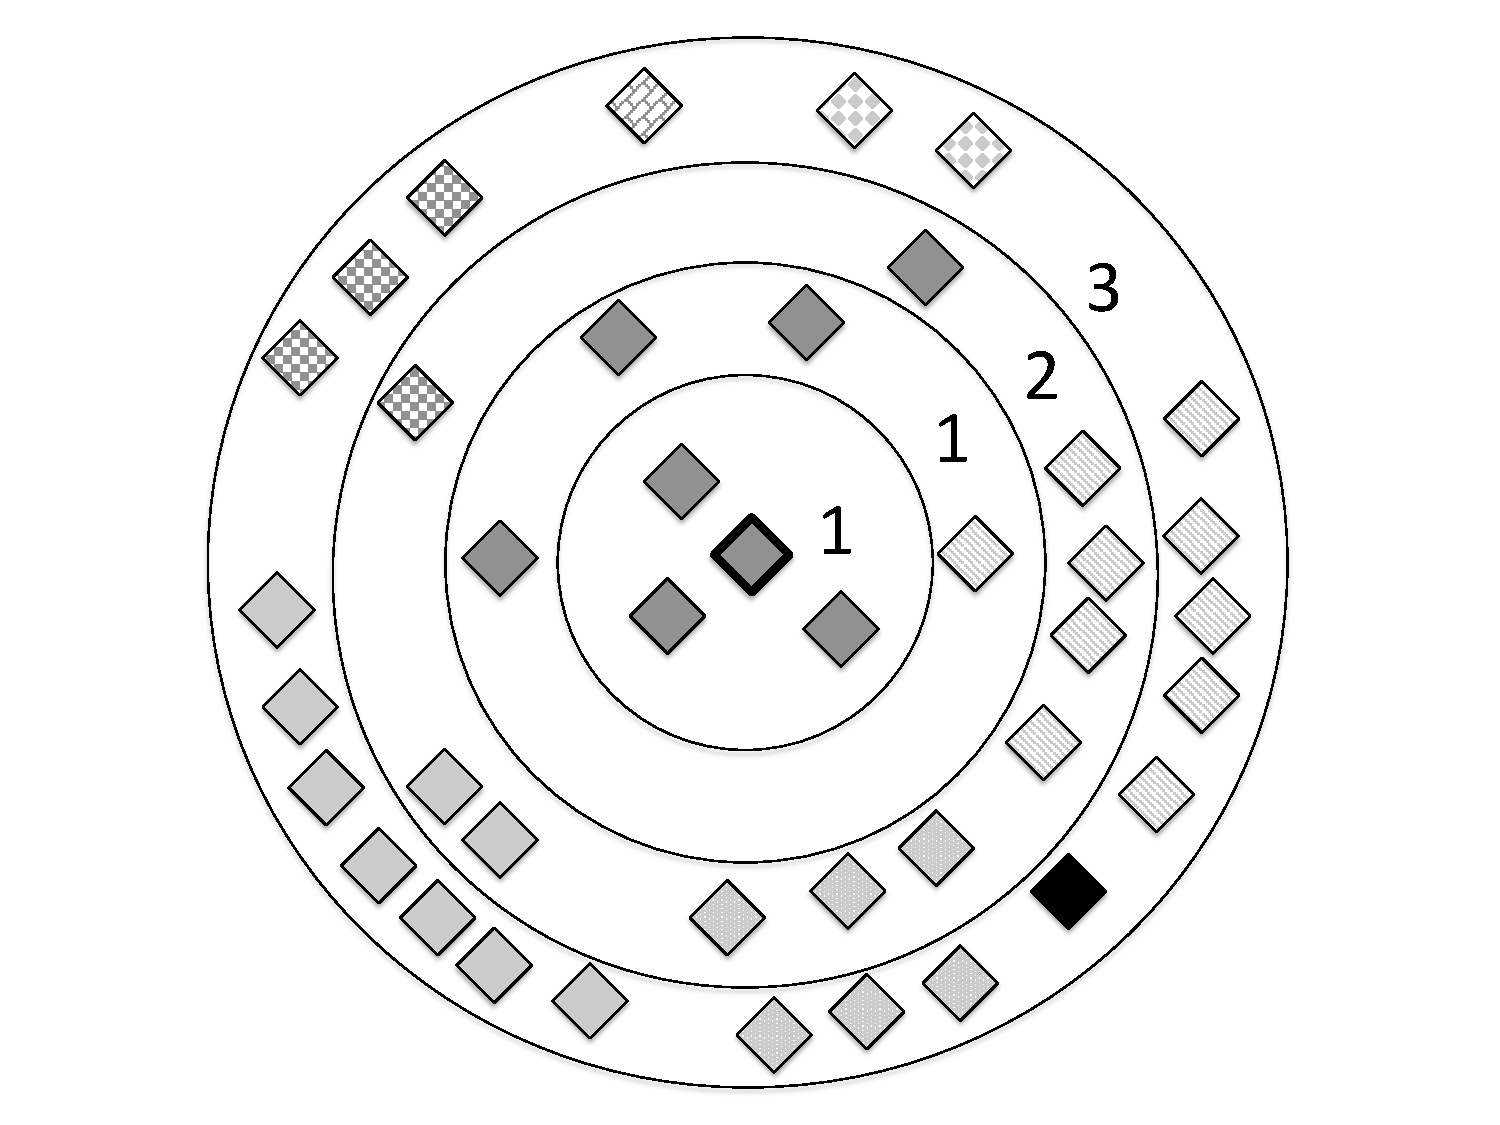
\includegraphics[width=0.4\columnwidth]{onionring}
\caption{\scriptsize{Onion-ring shows all repairs for the center-most test case, and all other test cases repaired by same mutants.  Rings represent repairing mutants, and diamonds test cases.  Diamond pattern symbolizes fault.  For innermost ring, all failures are due to the same fault.  As rings expand, the set of faults grows (as does distance).}}
\vspace{-0.1in}
\label{fig:onion}
\end{figure}

Consider the structure of mutants repairing a failure due to some optimization.  If many mutants repair this failure, by turning off the optimization or a whole family of optimizations, some will likely repair failures due to different faults.  Repairs naturally produce an \emph{onion-ring} structure (Figure \ref{fig:onion}), where a failure is repaired by (1) some mutants that are very specific to its fault (the inner rings) and repair few failures, as well as other mutants (2) that repair more and more faults, up to a hypothetical mutant (3) that turns off all optimization in the compiler (e.g., by effectively adding {\tt -O0}), the outer ring of the onion.  This does not introduce confusion, because the more repairs two tests have in common, the more likely they are to be due to the same fault, and the more they disagree on, the less likely they are to be due to the same fault.  While especially intuitive as a consequence of disabling compiler optimizations, it seems likely this structure appears for repairs in many programs.  Disabling an optimization is a code change that (usually) does not cause any test case that only concerns semantics, not speed, to fail, but can avoid some failures.  For some oracles, many changes may fall into this classification:  for example, if the only oracle is to detect crashes, a fault can be avoided by aborting the program early.  Turning off a data-structure invariant checker is another possible false repair that might cover many different faults.  In all these cases, assuming more interesting and specific ways to repair faults exist, a distance metric can still work.

The idea of measuring the distance between failures (or other test cases) by their response to mutants is appealing.  The most important aspect of most applications of distances between executions is some aspect of causality \cite{LewisCause,ZellerBook}.  Since at least the work of Hume \cite{Hume1}, causality has been understood as answering some question of the form ``what would have made a difference in this effect?''  A program mutant is a very direct way to answer this question.  The problem with determining causes of events in computer programs is that, as in most problems of causality, too many things can make a difference, most of which are not interesting.  Program mutants are much more likely to be interesting causes for events in a program than changes to test cases, at least for fault identification and debugging purposes, because the practical use of knowing a cause is to change the cause and avoid or produce an effect.  Debugging by changing test cases is not useful; debugging by altering the program is precisely how we seek to use the causes we discover.  Using mutants as causes in order to measure similarity ``inverts'' the ideas of Lewis \cite{LewisCause,LewisCount}, where similarity determines causality.  One pleasant side-effect is that execution representation \cite{NearNeighbor,RepsSpectra} is not a difficulty for this kind of metric, since an execution is always represented as a set of correctness evaluations.

This paper investigates the utility of using distance metrics based on the causal approach suggested above.  We show that such a metric can improve, in a statistically significant way, the ability to distinguish tests based on which faults they trigger.  Furthermore, fault localization based on the same metrics can successfully pinpoint the location of some compiler faults sufficiently to be likely to substantially aid debugging, and, when applicable, performs very well for some faults studied in recent papers on mutant-based fault localization \cite{multilingual,Papadakis}.

%\subsection{Contributions}

The contributions of this paper include our ideas about how to measure distance between program executions, but more importantly some practical proposals for using such a metric in compiler fuzzer taming and fault localization.  Our experimental results show that, for two realistic complex compilers, Mozilla's SpiderMonkey 1.6 JIT for JavaScript and GCC 4.3.0, using mutant response metrics improves FPF-based fuzzer taming over best previous results \cite{PLDI13}, in multiple ways.  Our fault localization approach also compares favorably to state-of-the-art fault localization techniques \cite{MUSE,multilingual,Metallaxis}, albeit with a more limited applicability (but also a lower cost).
\section{A Mutant-Based Distance Metric}

For every failing test case, the response (fixing or not fixing the
failure) to all mutants defines a bitvector, with
length equal to the number of mutants that repaired \emph{any} test
case (or all mutants; it does not matter for our proposed metric),
where a 1 bit indicates that the mutant in question repairs this test
case\footnote{By \emph{repairing} a failing test we here mean that a mutant
causes the test to pass, \emph{and} the mutant does not cause
other, previously passing tests, to fail.}.  These bitvectors cannot be effectively compared with Hamming distance. Consider $t_1$ and $t_2$, both repaired
by 100 mutants.  If these two test cases share 90 common repairing
mutants, and disagree for 10, they have a Hamming
distance of 20.  This makes them ``less similar'' than two test cases,
$t_1'$ and $t_2'$, where $t_1'$ is repaired by 5 mutants, $t_2'$ is
repaired by 5 mutants, and \emph{none of those mutants overlap.}   A Jaccard distance, also used (as similarity) in some fault
localization algorithms \cite{Pinpoint}, is a better fit.  For bitvectors $u$ and $v$ of length $n$:
%\vspace{-0.08in}
\[d(u,v) = 
\begin{cases}
\frac{\sum_{i=0}^{n-1} 1\ \text{if}\ u_i \neq v_i\ \text{else}\ 0}{\sum_{i=0}^{n-1} 1
\  \text{if}\ u_i \neq 0 \vee v_i \neq 0\ \text{else}\ 0} & \exists i:u_i\neq 0 \vee v_i\neq 0\\
0 & otherwise
\end{cases}
\]

\noindent In other words, the Jaccard distance is $\frac{\mathit{bitcount}(u
\veebar v)}{\mathit{bitcount}(u \vee v)}$ (the number of 1 bits in the
XOR over the number of 1 bits in the OR for $u$ and $v$); that is, the
distance is the portion of mismatches over repairing mutants for
either test.  This metric agrees with our intuitions about the above comparisons.  It
essentially formalizes the intuition of the onion-ring model, where
more matching repairs indicates a much higher probability two failures
are due to the same fault, even if not all repairs match.

Given such a metric, FPF \cite{Gonzalez} fuzzer taming \cite{PLDI13}
begins by ranking as first an arbitrary test case.   FPF next ranks the test
case, of all unranked tests, that has the largest minimum distance
from all ranked test cases --- the test case most dissimilar by \emph{closest}
already ranked test --- until all tests are ranked.  FPF is boundedly close
to optimal under certain assumptions \cite{Gonzalez}.

More complex metrics are possible, also combining information such as
coverage and language features or test case tokens \cite{PLDI13}.
However, mixtures of metrics (combining different features) other than
Levenshteins \cite{lev} over test case + output never performed well
compared to more focused metrics in earlier work \cite{PLDI13}.
Therefore, in order to evaluate the contribution of our repair-based
metric we compare it, alone, to the previous best metrics.

In Section \ref{conc} we discuss uses of $d$
requiring comparison of both failing and passing test cases:  in this 
case, we would use three-valued vectors, with a bit for each \emph{property}, where 1 indicates a 
failing property succeeds and -1 that a succeeding property 
fails.  For such an application, we could remove the requirement that
a repair not be a killed mutant, since the passing test vectors would encode
that information
\section{Localization and Explanation}

Automated fault localization \cite{FaultSurvey,Jones2002} provides users with
information about the likely location of a fault in a program's source
code.  Error explanation \cite{GroceError} also provides information
about the causal structure of a fault --- how it can be avoided, what
triggers it --- a kind of ``fault story.''  Parnin and Orso recently
suggested that fault localization methods are not actually providing a
great deal of assistance to real users in debugging \cite{AutoHelp}.
Automated fault localization has not been widely adopted in industry.

Parnin and Orso note that most popular methods are
statistical and tend to simply provide an ordered list of statements
to examine.  These statements are not guaranteed to be essentially
related to the fault --- with many techniques, the statements are,
too often, code that executes as a consequence of the fault, code
accidentally executed with the fault, and so forth.  Second, most
evaluations of fault localization have been performed over programs
where it is not clear that debugging is extremely hard, vs. the time
spent applying automated localization and establishing effective
(automated) testing to support automated localization.  Compiler
debugging, on the other hand, especially for subtle optimization-based
problems that produce incorrect code (vs. simple crashes) is generally
known to be difficult.
Researchers reporting subtle compiler bugs often observe the time from
reporting a fault to its correction, even once the fault is assigned,
to be lengthy, and the resulting patches are sometimes thousands of
lines \cite{PLDI13}.  Important compilers, whether JITs where security is paramount
or C compilers used to compile core systems code, also tend to already
be the
subjects of extensive automated testing \cite{jsfunfuzz,csmith}.

By definition, when a mutant repairs a test case, it changes the
behavior of the test.  In some cases, this behavioral change is
limited to changes in program state and data values.  However, the
vast majority of mutant repairs also modify the code coverage of a
test; in our experiments, there were no repairs that did not change
coverage.  If a fault can be avoided by, for example, disabling a
problematic optimization in a compiler, this naturally leads to
changed coverage.  If the fault is due to a bad conditional, where a
program path should include additional code, the repair will often
change the execution to include the omitted code.  As a localization
for a fault, then, we can examine the source statements whose
  coverage changed most often in repairs.  Early experiments with this
  approach showed that a useful coverage change localization must  account for the frequency of a
change.  Some coverage changes are extremely common across all
failures, faults, and repairing mutants,
and therefore likely not related to any specific fault.

\begin{quote}
The {\bf Coverage} localization for a failing test case $f$ in the set
of failures $F$ ranks
statements by the function $r$ (for rank) where:
%$$U = s : \forall m . \forall t \in F . c(m,t,s) = 1$$
$$C(s) = \sum_{t \in F} (\sum_{m \in R(t)} c(m,t,s))$$
%\[
$$r(s,f) = \sum_{m \in R(f)}\frac{1}{C(s)}c(m,f,s)$$
%\begin{cases}
% \sum_{m \in R(f)}\frac{1}{C(s)}c(m,f,s) & s \not\in U\\
%   0 & s \in U
%\end{cases}
%\]
$c(m,t,s)$ is 1 if coverage of $s$ changes for test $t$
with mutant $m$, and 0 otherwise.  $R(f)$ is the set of mutants repairing $f$.
\end{quote}

That is, the ranking is based on the number of times a statement's
coverage changes its value (covered or not covered) from the original
execution of $f$ in executions of mutants that repair $f$.  Changes are weighted by their inverse frequency over all
failures and all mutants.
Higher values for $r$ result in a higher ranking (more likely to
be faulty).  
%Computing $U$ accounts for the fact that in our
%experiments, a few statements were added or removed for every single
%r

The repairing mutants themselves can also be used for localization and
explanation.  While few will be equivalent to actual fixes, they
will sometimes overlap the incorrect code, and will often be closely
related to incorrect code, semantically.  Since many failures are
fixed by a large number of mutants, it is important to rank the
mutants to produce a localization.  Based on the onion-ring model proposed above, this is simple: each mutant is ranked as
a localization/explanation based on the \emph{most distant failure it also
  repairs.}  If a given mutant only repairs failures that have similar
repair vectors to the test case being localized, it will be highly
ranked.  If it repairs even one very dissimilar failure, then it will
be considered a poor localization.

\begin{quote}
The {\bf Repair} localization for a failing test case $f$ ranks
statements by the function $r$ where:
%$$dmax(m,f) = max_{t : m \in R(t)} d(t,f)$$
\[
r(m,f) = 
\begin{cases}
\frac{1}{1 + max_{t \in F: m \in R(t)} d(t,f)} & m \in R(f)\\
0 & m \not\in R(f)\\
\end{cases}
\]
%$$\text{leastfar} = m \in R(f) : \neg\exists m' : \text{far}(m',f) <
%\text{far}(m,f)$$
\end{quote}

This ranks a mutant $m$ (and associated statement) by the inverse of the distance
from $f$ to the most distant failng test also repaired by $m$, adding 1
so that if $m$ only repairs failures at distance 0 $r$ is well defined
(and maximal).
If $m$ does not repair $f$, it is not ranked at all.  One advantage of
this approach over some statistical methods is that by
ranking \emph{mutants} the localization offers developers not simply a
ranked statement but a kind of ``explanation'' \cite{GroceError} of the fault:  if \emph{this
mutant} were applied, the fault would not exhibit.  As Kochhar et
al. show \cite{Kochhar}, a large majority (more than 85\%) of developers considered
the ability of a localization tool to provide a \emph{rationale} or
reason for a localization important.  A mutation plus the tests that
stop failing when it is applied is a practical, concrete explanation
of a fault localization.  Mutants that repair a failure provide insight 
into the nature of the fault, and, we hypothesize, more information the 
closer they are to the center of the onion-ring. 

The coverage localization also provides a kind of explanation, though
a less direct one.  For any
interesting line of code in the coverage-change-based localization,
the user can investigate a particular instance of the change,
by selecting a single mutant and stepping through the execution of the
failing test case in a debugger to the point of change.  The user can also
browse through all mutants that produce this coverage change for the test
case.  

Another advantage over many statistical approaches to
localization is that our methods are not potentially confused in
settings with multiple faults.  Each localization/explanation is based
on a single failing test case, which in most cases fails due to only one
fault.  In fact, other faults help both methods rank localizations.
\section{Experimental Results}

\begin{figure*}[t!]
    \centering
    \begin{subfigure}[t]{0.5\textwidth}
        \centering
        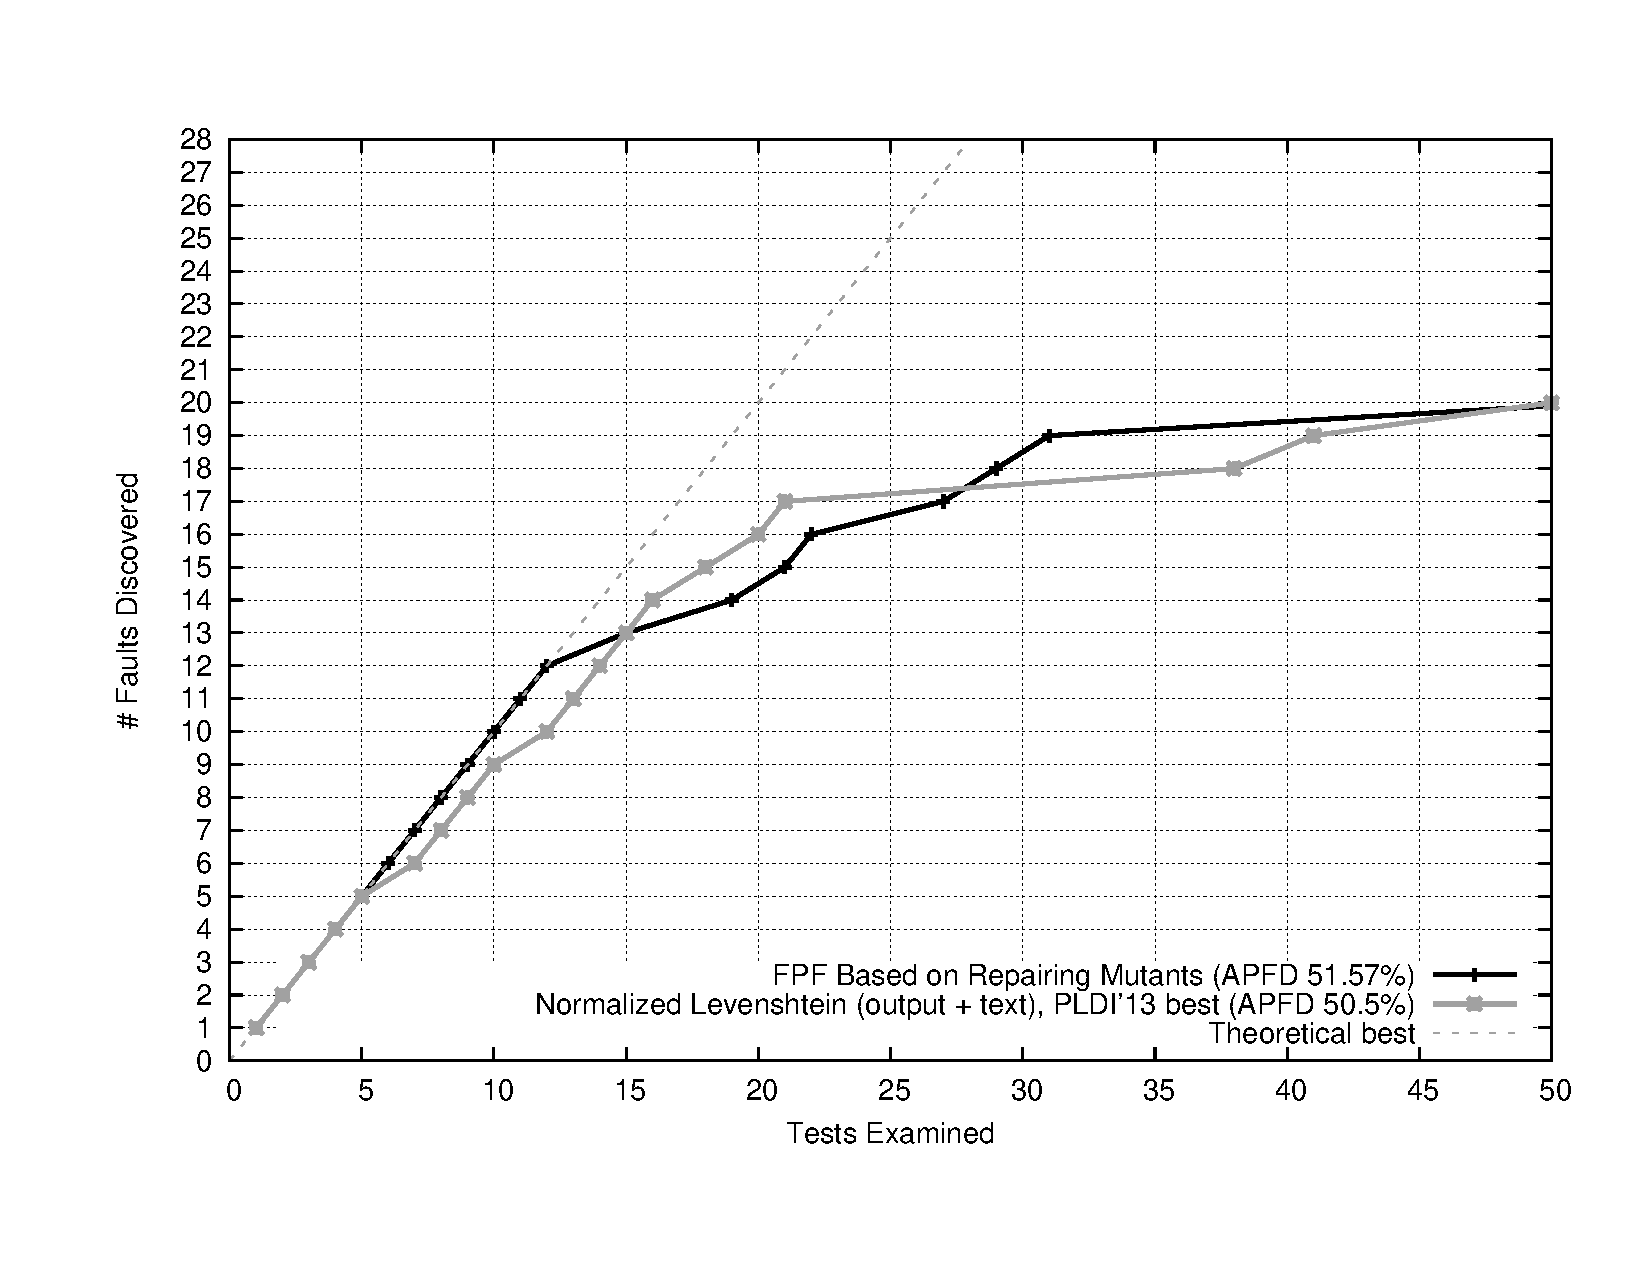
\includegraphics[width=1.0\textwidth]{jscurve}
        \caption{Discovery curves for SpiderMonkey 1.6 faults}
        \label{jscurves}
    \end{subfigure}%
    ~ 
    \begin{subfigure}[t]{0.5\textwidth}
        \centering
        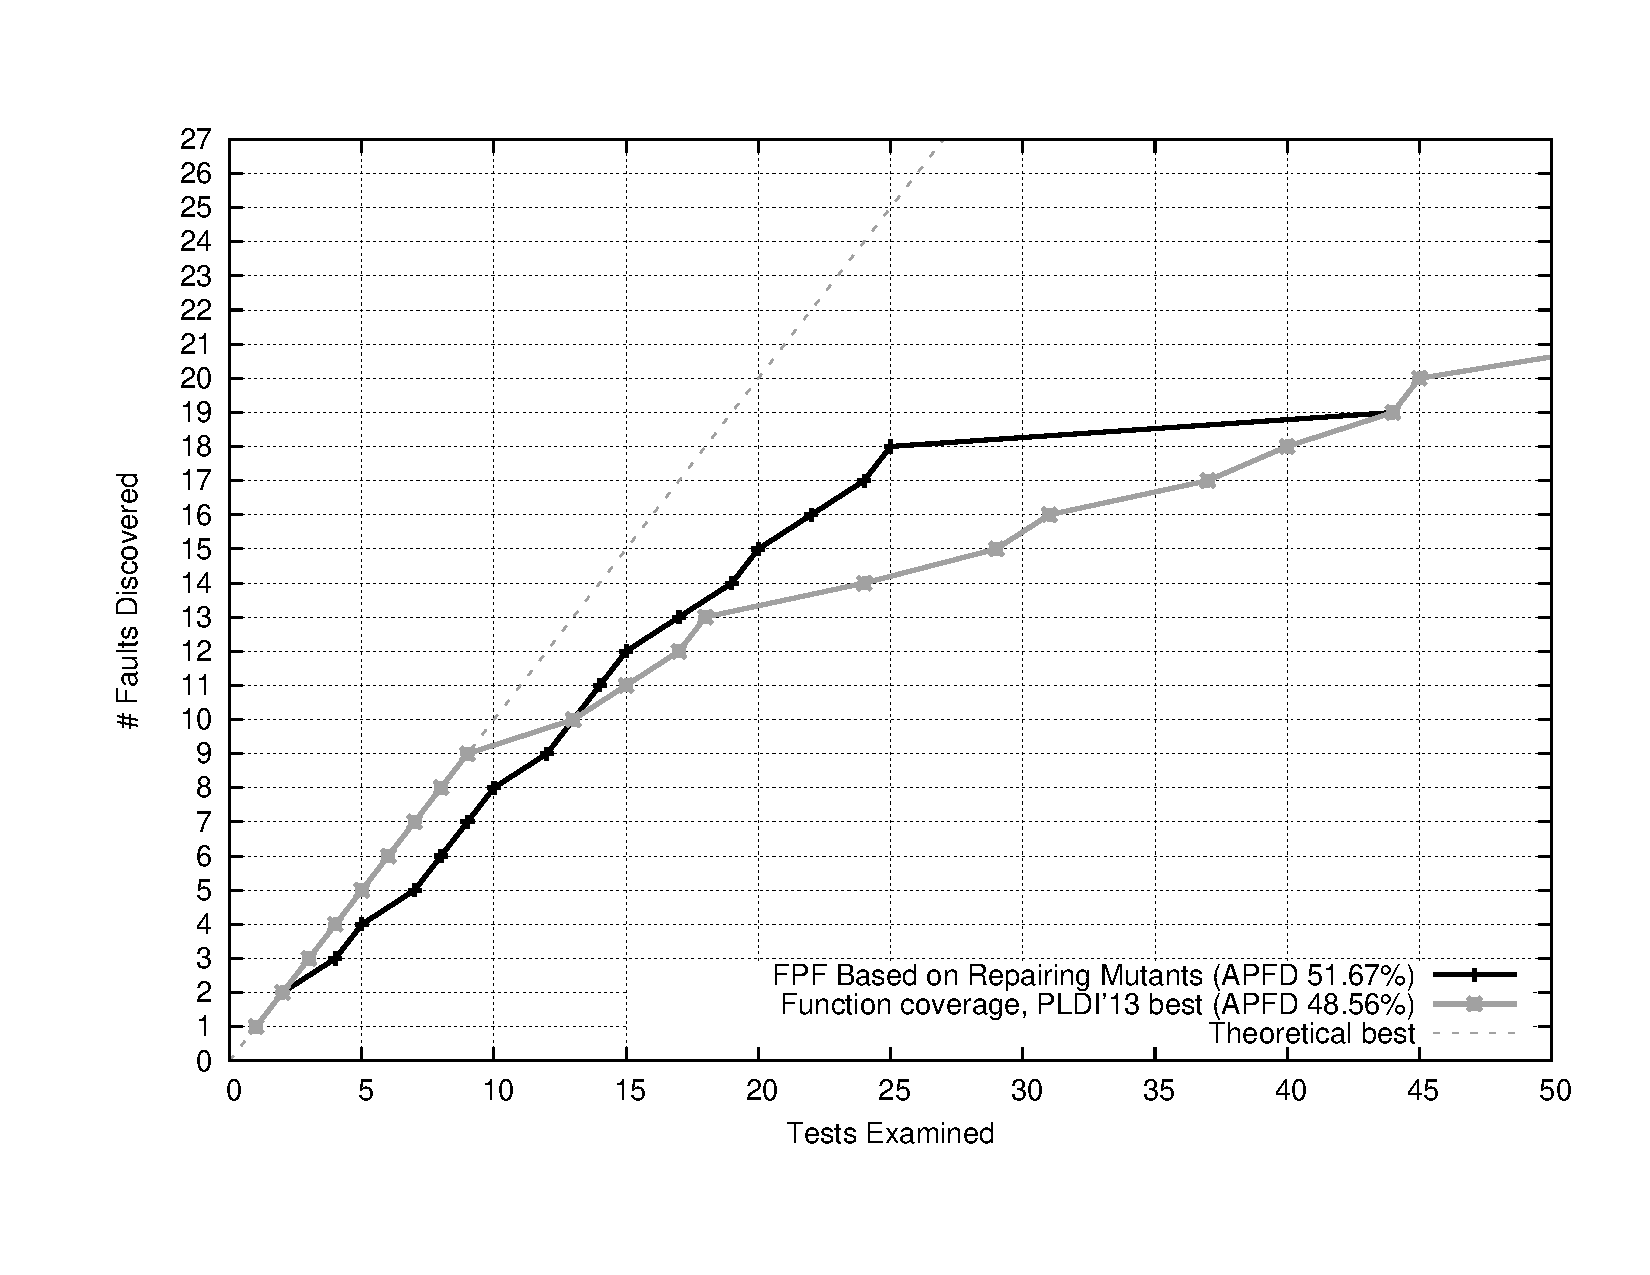
\includegraphics[width=1.0\textwidth]{gcccurve}
        \caption{Discovery curves for GCC 4.3.0 wrong-code faults}
        \label{gcccurves}
    \end{subfigure}
    \caption{Discovery curves compared to best curves from PLDI 2013}
\end{figure*}


%\begin{figure*}
%\centering
%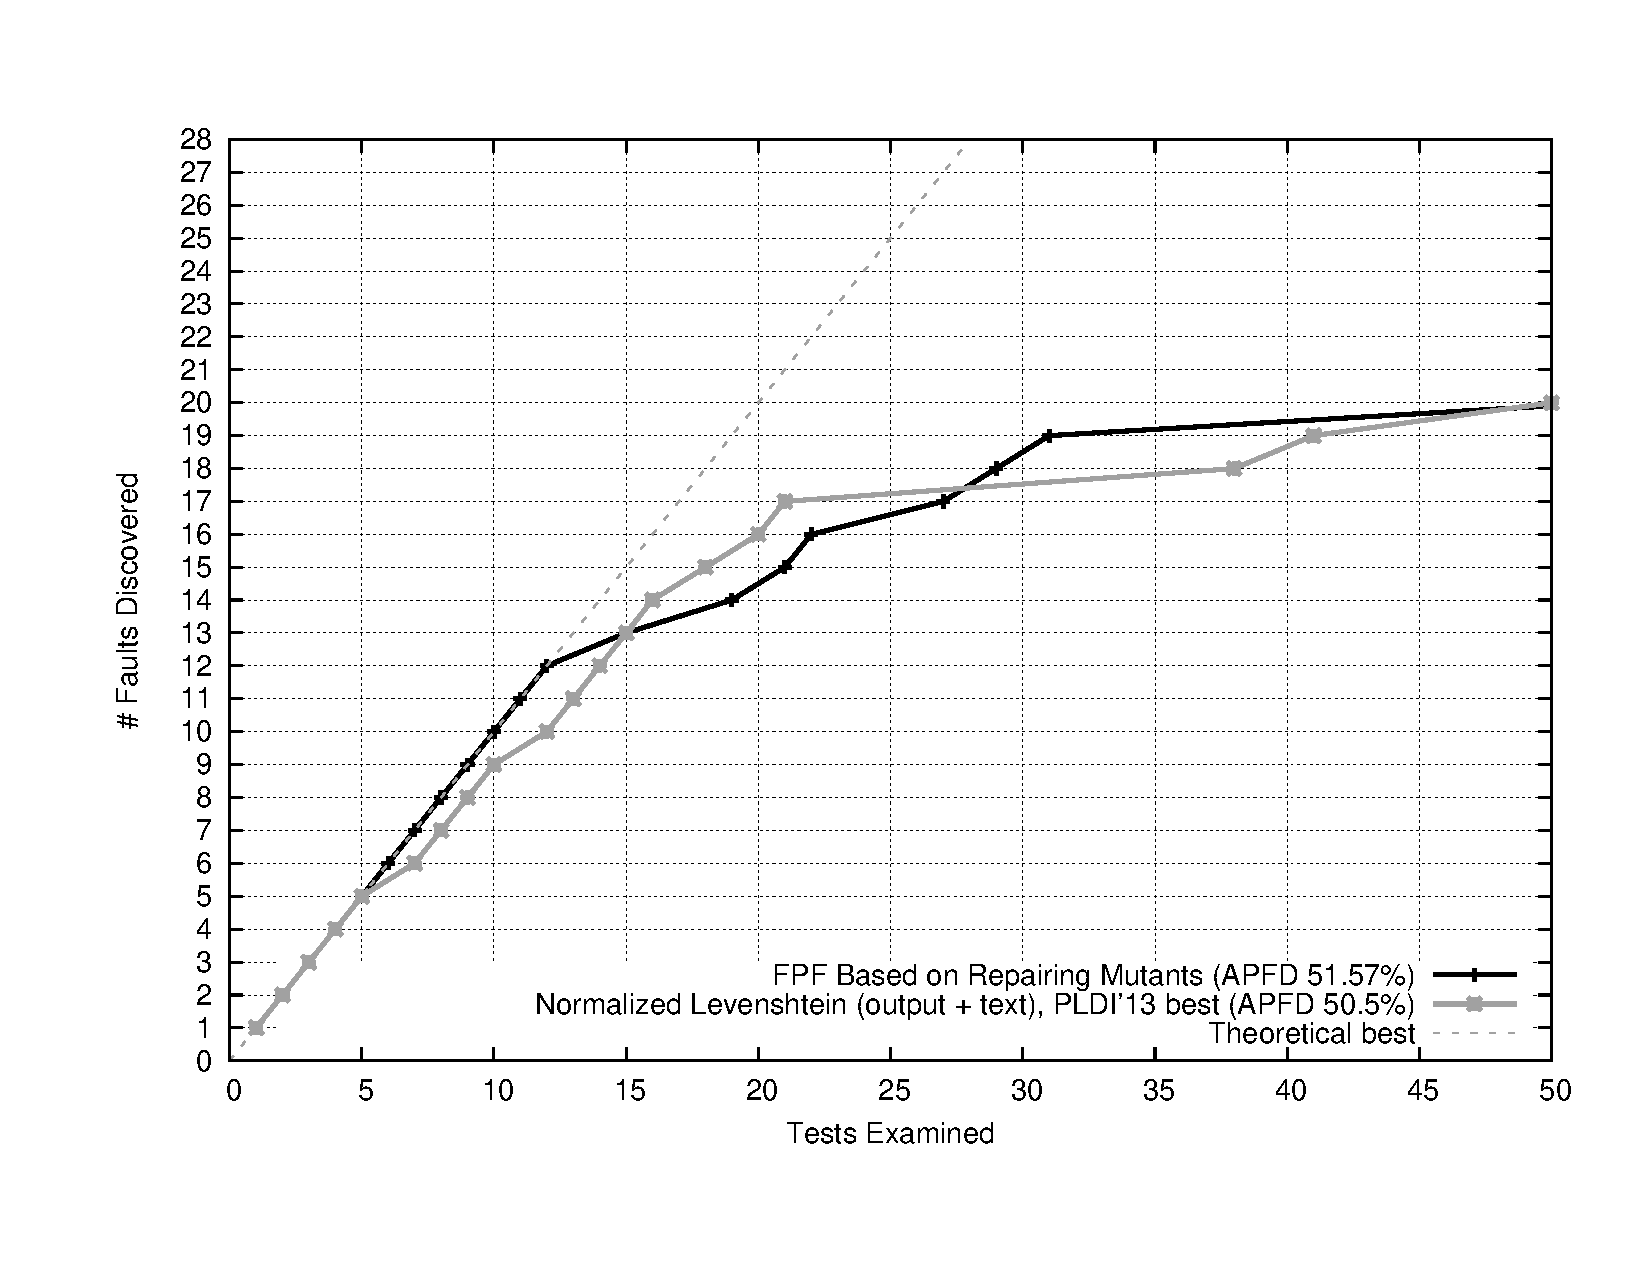
\includegraphics[width=2\columnwidth]{jscurve}
%\caption{Discovery curves for SpiderMonkey 1.6 faults}
%\label{jscurves}
%\end{figure*}


%\begin{figure*}
%\centering
%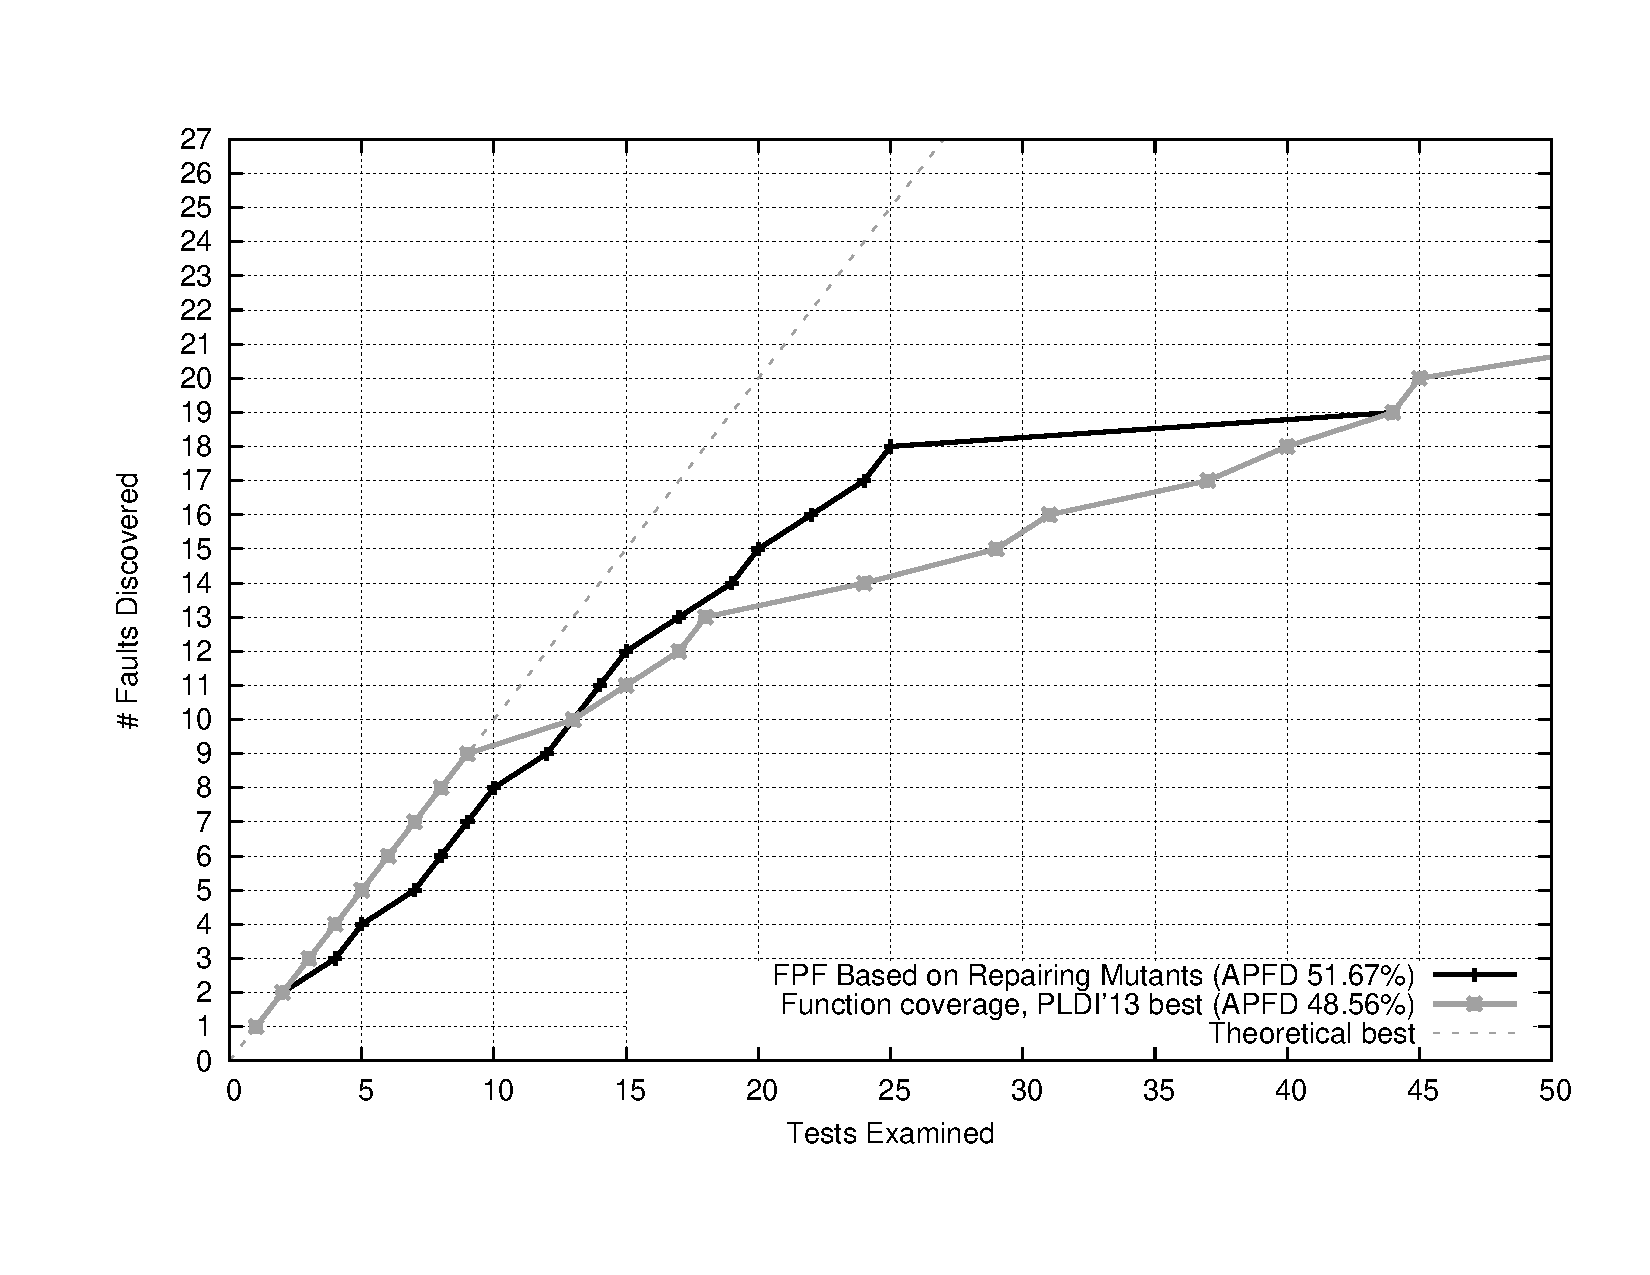
\includegraphics[width=2\columnwidth]{gcccurve}
%\caption{Discovery curves for GCC 4.3.0 wrong-code faults}
%\label{gcccurves}
%\end{figure*}

%\subsection{General Experimental Framework}

Our primary experiments are based on subjects used in the only previous study of compiler fuzzer taming \cite{PLDI13}.  Of the three data sets examined in that paper, this paper considers two:  faults and tests cases for SpiderMonkey 1.6, Mozilla's JavaScript engine, with tests generated by {\tt jsfunfuzz} \cite{jsfunfuzz}, and \emph{wrong code} faults and test cases for GCC 4.3.0, with tests generated by Csmith \cite{csmith}.  GCC 4.3.0 crash faults were essentially perfectly localized by previous approaches.  In fact, on examination, only two of the 11 crash bugs are not distinguished by simply examining the crash message.  Faults that produce a crash are also likely to be much easier to debug than semantic problems such as all of the GCC wrong code bugs and most of the JavaScript faults --- e.g., following a dynamic slice might well suffice.

\comment{
We applied our metric to two of the datasets used in the previous study of compiler fuzzer taming \cite{PLDI13}: faults and tests cases for SpiderMonkey 1.6, Mozilla's JavaScript engine, with tests generated by {\tt jsfunfuzz} \cite{jsfunfuzz}, and \emph{wrong code} faults and test cases for GCC 4.3.0, with tests generated by Csmith \cite{csmith}.   We did not use the crash faults from that data set, as these are in practice fairly easy to identify by hand (and perfectly identified by previous metrics), and also typically easy to debug.  }

Our mutants were produced using the tool written by Jamie Andrews \cite{mutant}.  Andrews' tool applies only four operators: statement deletion, conditional negation, operator replacement, and constant replacement, chosen as a small set that still produces good results for C code.  Experiments were performed on a MacBook Pro with 16GB RAM and dual-core 3.1GHz Intel Core i7; GCC executed on a VirtualBox-hosted Ubuntu 11.04.  For GCC, some test cases from the 2013 PLDI paper no longer failed, presumably due to unknown differences in execution environment, OS, or memory layout. Discarding these reduced the set of test cases from 1,275 to 1,117 and the number of distinct faults to 27 rather than 35.  For SpiderMonkey, all 1,749 test cases from the PLDI 2013 data failed in the new environment, representing 28 distinct faults.

These data sets, though similar in that both compilers are written in C, provide some interesting variance for testing our metrics.  The oracle for SpiderMonkey executions is the set of checks built in to {\tt jsfunfuzz} plus the requirement that the execution not crash.  This is only a moderately strong oracle, and allows serious deviations from both the JavaScript language specification and normal SpiderMonkey behavior, while checking some complex details, such as {\tt eval} round-trips.  For GCC, the oracle is a differential check on a hash code:  failure was defined as producing a executable with the -O3 flag that, when executed, produced a different checksum than code compiled by either of GCC 4.9.3 or clang 7.0.0, both using -O0.  A repairing mutant must enable GCC 4.3.0 to actually compile code correctly, which is a very strict correctness property, making coincidental correctness \cite{CCT} highly unlikely --- only missed optimizations are allowed.

We only show results for the first 50 tests in the ranking, and computed areas under curves for the same limit, since it seems very unlikely that a user will examine many more than 50 tests, especially given the decreasing slope of the discovery curves.  In practice, after 50 tests, fixing a few faults and then re-running tests and FPF seems the most likely recourse, and we confirmed that after removing random subsets of faults, our metrics still outperform the previous best.  We applied X-means \cite{xmeans} in an attempt to use clustering with our metrics, but, as with previous results \cite{PLDI13} it did not compare well with FPF, and the runtime was much higher.  We confirm the conclusion \cite{PLDI13} that clustering is of limited value in fuzzer taming.
% (at least with X-means) does not work well in a setting with extreme disparity in instance counts for faults.  %A further difficulty for our setting is that X-means and most off-the-shelf clustering tools take vectors, not a distance metric.  X-means is using the raw repair data, not weighted by the fact that 0-0 agreement is much less informative than other possible matchings (a Euclidean over 0-1 vectors is just the square root of Hamming distance).

\subsection{Mozilla SpiderMonkey 1.6 Results}


There were 96,828 SpiderMonkey mutants, based on 69,634 lines of code in C and header files.  Of these mutants, 12,666 were covered by some failing test case.  Of these mutants, 10,525 survived a basic set of SpiderMonkey quick tests \cite{icst2014}.  Of these mutants, 1,326 (12.6\%) repaired at least one test case.  Figure \ref{jscurves} shows the discovery curves for the mutant repair metric compared to the ideal discovery curve and the best curve from previous work using FPF, which used a normalized Levenshtein distance \cite{lev} over the failure output and test case text \cite{PLDI13}.  A discovery curve is a plot of the number of distinct faults that a user, examining the tests in the ranked order, would have seen after N tests (here, N goes up to 50).

The APFD (Average Percent Faults Detected) values in the graphs are based on the measure  introduced by Rothermel et al. for evaluating test case prioritization methods \cite{APFD}.  APFD is a somewhat better summary of results than the raw curve areas used for evaluation in previous work \cite{PLDI13}.  APFD, as the name suggests, measures the percent of all faults discovered at the ``average'' point on the curve, by comparing the curve's area to an ideal curve, with interpolation.  A simpler (but less informative) way to compare the curves is to note that the mutation-based metric's curve is above the best previous curve at 60\% of data points.
%\footnote{The details of APFD calculation are slightly involved, and the interpolation and perfect curve are not exact fits for fuzzer taming; nonetheless the basic method summarizes curves fairly well and is standard in the testing literature for similar problems \cite{issta14}.}. 

APFD results are useful summaries, but the curve itself is also worth examining, since (1) long sequences of tests with no new faults may discourage users more than an overall less effective but steadily climbing curve with few ``plateaus'' as we call these uninformative sequences of tests and (2) a good early curve is important to developers.  The mutant repair curve climbs very rapidly in the early portion, with perfect discovery for the first 12 faults. The largest plateau is 5 tests without a new fault, ignoring the long period after the 31st test.  In fact, a plateau at the end of the curve is not problematic.  Assuming that few users will examine more than 50 test cases without fixing some faults, the user may give up after seeing 10 or more tests without a new fault based on the mutant repair curve, and in fact lose nothing by doing so.  The PLDI 2013 curve, in contrast, has a plateau of size 17 after the 17th fault.  If we assume a user stops examining tests after a size 10 or greater plateau, the user will only see 17 faults using the PLDI 2013 metric, vs. 19 with our metric.  Stopping at a plateau of size 6 produces the same results.

Over all mutants, and all pairs of test cases repaired by the same mutant (so the same pair may count many times, if many mutants repair both test cases), the probability of being due to the same fault was 42.77\%, and the probability of being due to the same fault if two test cases disagreed on a repair (the mutant repaired one test case but not the other) was only 20.33\%.  The baseline rate for same-fault for test pairs was 33.64\%.  Just knowing that two test cases have \emph{one} shared repairing mutant makes it 1.27x more likely that they are the same fault, and knowing they differ for one mutant makes it 0.6 times as likely they are due to the same fault.  Matching non-repair, however, provides very weak evidence:  only a 34.14\% chance of matching fault, just over baseline.

An additional measure of effectiveness is to consider how effective a metric is in producing matched nearest neighbors.  That is, how often is the nearest neighbor of a failure (that is not due to a singleton fault --- a fault detected by only one test case) due to the same fault?  For reduced \cite{DD,PLDI13,
CReduce} test cases, we assume that for a perfect metric, the nearest neighbor should almost always share the same fault, since there is little or no extraneous semantic content to each test beyond the cause of failure.  For the SpiderMonkey failures, 96.3\% of non-singleton failures matched their nearest neighbor(s).  For mutants that repaired any failures, the mean and median number of test cases repaired were 120.6 and 4.0, respectively.  Most mutants repaired a small number of tests, but a few mutants repaired a very large number of tests.  A few mutants repaired \emph{all} SpiderMonkey faults; obviously these mutants were not actual fault fixes, but effectively disabled some mechanism {\tt jsfunfuzz} used to detect failure. The mean and median homogeneity for repairing mutants (\% of failures repaired corresponding to the most common fault repaired) were 77.96\% and 86.36\%, respectively.  

In order to check our results statistically, we sliced the PLDI 13 tests into 20 randomly selected equal-sized (as much as possible) distinct subsets.  The repair metric had a mean APFD (89.23\%) for these subsets that was 2.85\% better than the mean APFD for the PLDI 13 metric (86.76\%), over sets of $\sim 10$ faults. The result was statistically significant ($p < 0.05$ by Wilcoxon test).   Median repair APFD was 90.05\%, vs. 84.75\% for PLDI 13's best metric.


\subsubsection{Fault Localization}

Table \ref{bothtable} shows a comparison of three fault localization methods for the SpiderMonkey (and GCC) faults.  The first column is a fault ID. The next three columns show localization rankings.  A dash for a column means that localization did not rank any faulty statements, or assigned all faulty statements suspiciousness of 0.0.  The three rankings are: our {\bf Repair} localization, the MUSE \cite{MUSE} localization, and the MUSEUM \cite{multilingual} localization, which uses the same formula as MUSE, but works better for multiple faults because it uses only one failure.  The MUSE/MUSEUM formulas normally make use of information from passing tests as well: when mutating a statement makes a passing test case fail, it makes the statement \emph{less} suspicious, by a weighted amount. The weight assigned to information from passing tests in our setting would likely be low (due to the ratios of repairs to mutation kills).  In a limited sense, information from passing tests is already incorporated in our results.  Throwing out all mutants that are killed by any passing test as potential repairs/localizations ensures that the rankings of all statements that are in MUSE/MUSEUM rankings are correct, \emph{relative to each other}.  By definition, passing tests have no influence on the suspiciousness of these mutants.  However, there may be other mutants that 1) repair a failure and 2) are killed by some test case: these could, if enough different ones repaired the same faulty statement, improve MUSE/MUSEUM results, though in practice this is extremely unlikely.  We reject such mutants in part to keep costs low, and in part because we think that the causal information contained in such mutants, that ``fix'' a failure but also break some passing test(s), is problematic.  They seem likely to be less useful as explanations of the causes of a failure, since they do not impact the program semantics in a way that is only known to be beneficial, and could potentially even mislead a user if used as explanations.  \comment{Still, it is most useful to compare MUSEUM/MUSE and our approach on the cases where all methods produce a localization.}

Discussion with the MUSE/MUSEUM authors confirms  that adding information for passing tests, while costly, would likely improve the MUSE and MUSEUM results, given the weakness of our oracles, particularly for SpiderMonkey, and should be considered essential for ideal application of their approach.  Because the cost of recording the full mutant analysis matrix for all passing tests (rather than considering a mutant killed as soon as one test fails, as we do) is very high, and we would like to produce a comparison over a fixed computational cost, we give results for MUSE/MUSEUM over failing tests only, cautioning that we are not sure what the impact of this choice is on faults that were not localized.  For similar reasons of keeping costs low, we also used the mutation operators of Andrews vs. the more extensive Proteum \cite{Proteum} operators used in MUSE/MUSEUM's evaluations.  \comment{Even with these restrictions, running all mutants on passing tests until at least a single kill was observed took about 3 times as long as the search for repairs, which we already consider a potentially problematic cost.}  In Section \ref{sec:otherfaults} we provide some comparisons with MUSEUM and MUSE fault localization in the context of a full mutation result matrix using their preferred set of operators.

\comment{
Results are reported as absolute ranks, rather than more sophisticated \cite{MUSE} localization evaluations because our localizations do not assign suspiciousness scores, only rankings, and in accord with the proposal of Parnin and Orso that only localizations ranking a fault in the top few statements may be useful to users \cite{AutoHelp}.  We expect users to examine coverage changes and mutants.  Blind, unaided pointers to portions of compiler code without more semantic information about why the statement is suspicious seem unlikely to work well, based on our experience with complex compiler faults, and the results of Parnin and Orso \cite{AutoHelp}.
}

\comment{
\begin{table}
\centering
{\scriptsize
\begin{tabular}{|c||c|c|c|}
\hline
%& \multicolumn{3}{|c|}{Localization Rank} \\
%\hline
Fault & Repair & MUSE & MUSEUM \\
\hline
880 & - & - & - \\
95 & - & 173 & -\\
1294 & 1 & 22 & 4 \\
60 & - & - & -\\
1543 & 19 & 118 & 26\\
1172 & 28 & 87 & 23\\
1561 & - & - & - \\
115 & 3 & 133 & 5 \\
\hline
\end{tabular}
}
\caption{Fault localization results for SpiderMonkey}
%\vspace{-0.2in}
\label{jstable}
\end{table}
}

%%%%%%%%%%%%%%%%%%%%%%%%%%%%%%%%%%%%%%%%%%%%%%%%%%%%%%%%%%%%%%%%%
% \begin{comment}                                               %
% \begin{figure}                                                %
% {\scriptsize                                                  %
% \begin{code}                                                  %
% {\bf Diff of old ($<$) vs new ($>$) for 115 patch (portion):} %
% ...                                                           %
% <             vp[1] = OBJECT\_TO\_JSVAL(thisp);               %
% <         \} else \{                                          %
% <             ok = OBJ\_GET\_PROPERTY(cx, thisp, id, \&v);    %
% <         \}                                                  %
% ...                                                           %
% <                   a->avail = (jsuword)sp;                   %
% <               \}                                            %
% ...                                                           %
% ---                                                           %
% >         RESTORE\_SP(fp);                                    %
% ...                                                           %
% {\bf Mutant information:}                                     %
% Failure repaired by 148 mutants.                              %
% ...                                                           %
% \#3: delete statement mutant of jsinterp.c:944:               %
%                                                               %
%             vp[1] = OBJECT\_TO\_JSVAL(thisp);                 %
%         \} else \{                                            %
% /*MUTANT    ok = OBJ\_GET\_PROPERTY(cx, thisp, id, \&v);*/    %
%         \}                                                    %
%                                                               %
% {\bf Coverage change information:}                            %
% ...                                                           %
% \#6: 5 mutants (3.38\% of repairs) added jsinterp.c:992:      %
%                    a->avail = (jsuword)sp; /* ADDED */        %
% \end{code}                                                    %
% }                                                             %
% \caption{Patch and explanation for fault 115}                 %
% %\vspace{-0.18in}                                             %
% \label{fig:explain}                                           %
% \end{figure}                                                  %
% \end{comment}                                                 %
%%%%%%%%%%%%%%%%%%%%%%%%%%%%%%%%%%%%%%%%%%%%%%%%%%%%%%%%%%%%%%%%%

Table \ref{bothtable} only includes 8 of the 28 SpiderMonkey faults.  This is due to a problem with the data set:  producing ground truth patches for a large application, in the sense of finding a minimal, clearly fault-fixing code change that can be back-ported to the original code is difficult \cite{PLDI13}.  While we believe the 28 faults identified in the PLDI 2013 data set are correct, it is very difficult to produce a valid patch of version 1.6 that captures the fix for most of these faults.  In some cases the final commit that caused tests to stop failing appeared to only be the end of a complex series of changes that converged on a correct fix.  In other cases, the code was modified so extensively before the fix that identifying ``the incorrect part'' of the original code seemed to owe more to guesswork than certainty.  The evaluation of localization therefore only examines the 8 faults for which we could be reasonably certain that the patch to 1.6 was correct and characterized the fault in question accurately.  In no case was the patch equivalent to one of the mutants (the smallest patch modified two statements).

No method performs extremely well --- for half the faults, no methods produced what we consider a useful localization.   Compiler faults are hard to debug, and any help is useful, but it seems unlikely developers will really benefit from a localization when it does not rank at least one faulty statement in the first 25-30 statements.  By this measure, MUSE only provides a helpful localization once, and performs worst of the methods.  {\bf Repair} and MUSEUM both perform well, with {\bf Repair} slightly better.

%%%%%%%%%%%%%%%%%%%%%%%%%%%%%%%%%%%%%%%%%%%%%%%%%%%%%%%%%%%%%%%%%%%%%%%%%%%%%%%%%%%%%%%%%%%%%%%%%%%%%%%%%%%%%%%%%%%%%%%%%%%%%%%%%%%%%%%%%%%%%%%%%%%%%%%%%%%%%%%%%%%%%%%%%%%%%%%%%%%%%%%%%%%%%%%%%%%%%%%%%%%%%%%%%%%%%%%%%%%%%%%%%%%%%%%%%%%%%%%%%%%%%%%%%%%%%%%%%%%%%%%%%%%%%%%%%%%%%%%%%%%%%%%%%%%%%%%%%%%%%%%%%%%%%%%%%%%%%%%%%%%%%%%%%%%%%%%%%%%%%%%%%%%%%%%%%%%%%%%%%%%%%%%%%%%%%%%%%%%%%%%%%%%%%%%%%%%%%%%%%%%%%%%%%%%%%%%%%%%%%%%%%%%%%%%%%%%%%%%%%%%%%%%%%%%%%%%%%%%%%%%%%%%%%%%%%%%%%%%%%%%%%%%%%%%%%%%%%%%%%%%%%%%%%%%%%%%%%%%%%%%%%%%%%%%%%%%%%%
% \begin{comment}                                                                                                                                                                                                                                                                                                                                                                                                                                                                                                                                        %
% \subsubsection{Error Explanation}                                                                                                                                                                                                                                                                                                                                                                                                                                                                                                                      %
%                                                                                                                                                                                                                                                                                                                                                                                                                                                                                                                                                        %
%                                                                                                                                                                                                                                                                                                                                                                                                                                                                                                                                                        %
% Figure \ref{fig:explain} shows part of the patch for SpiderMonkey fault 115, and the {\bf Coverage} and {\bf Repair} outputs that successfully localize the fault (the 6th coverage change output, and the 3rd mutant output), to give some idea of the information our methods present.  For {\bf Coverage}, it is surprising that the sixth highest ranked change only appeared in 5 of 148 repairs. This change ranked high out of thousands of changes because it was unusual, appearing for only 10 repairs in the entire SpiderMonkey analysis.  %
%                                                                                                                                                                                                                                                                                                                                                                                                                                                                                                                                                        %
% The precise form an explanation based on our techniques should take is not clear.  One possibility, suggested by the results here, is a method focused on repairs, but using common coverage changes.  For each repairing mutant, in rank order, the highest ranking coverage changes for that mutant could also be shown, to give an idea of unusual (and potentially localizing) changes induced by repair.                                                                                                                                          %
% \end{comment}                                                                                                                                                                                                                                                                                                                                                                                                                                                                                                                                          %
%%%%%%%%%%%%%%%%%%%%%%%%%%%%%%%%%%%%%%%%%%%%%%%%%%%%%%%%%%%%%%%%%%%%%%%%%%%%%%%%%%%%%%%%%%%%%%%%%%%%%%%%%%%%%%%%%%%%%%%%%%%%%%%%%%%%%%%%%%%%%%%%%%%%%%%%%%%%%%%%%%%%%%%%%%%%%%%%%%%%%%%%%%%%%%%%%%%%%%%%%%%%%%%%%%%%%%%%%%%%%%%%%%%%%%%%%%%%%%%%%%%%%%%%%%%%%%%%%%%%%%%%%%%%%%%%%%%%%%%%%%%%%%%%%%%%%%%%%%%%%%%%%%%%%%%%%%%%%%%%%%%%%%%%%%%%%%%%%%%%%%%%%%%%%%%%%%%%%%%%%%%%%%%%%%%%%%%%%%%%%%%%%%%%%%%%%%%%%%%%%%%%%%%%%%%%%%%%%%%%%%%%%%%%%%%%%%%%%%%%%%%%%%%%%%%%%%%%%%%%%%%%%%%%%%%%%%%%%%%%%%%%%%%%%%%%%%%%%%%%%%%%%%%%%%%%%%%%%%%%%%%%%%%%%%%%%%%%%%


\subsection{GCC 4.3.0 Wrong Code Results}


\begin{figure}
  \centering
  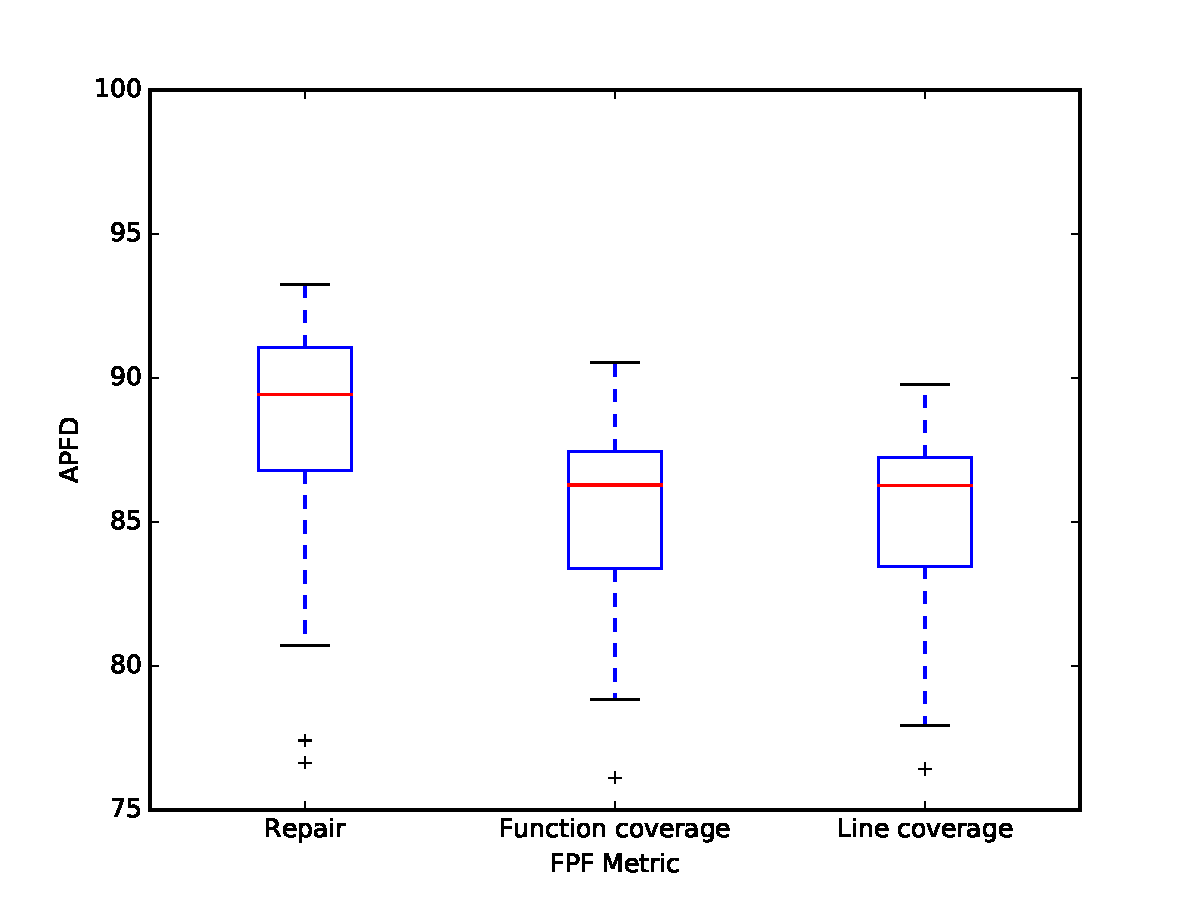
\includegraphics[width=0.8\columnwidth]{comparegcc}
  \caption{APFD values for GCC suite slices}
  \label{comparegcc}
\end{figure}%

There were 377,679 GCC mutants, based on 424,186 lines of code in C and header files. Of these mutants, 73,016 were covered by some failing test case.  Of these mutants, 41,385 survived a GCC bootstrap build, compiled hello world, and passed a GCC test suite.  Of these mutants, 3,232 (7.8\%) repaired at least one test case.  Figure \ref{gcccurves} shows discovery curves for the mutant repair metric vs. the best PLDI 2013 curve, Euclidean distance over function coverage vectors \cite{PLDI13}.  GCC's APFD improvement is larger than that for SpiderMonkey, but its early curve (first 15 tests) is worse compared to the PLDI 2013 curve, but still has a maximum gap of only 2 redundant tests vs. 4 for PLDI 13.  Over all, again the curve is better than the best PLDI 13 curve at 60\% of all points.  Using the hypothetical model where a user stops examining tests after a plateau of size 10, the user of the mutant-based taming will see 18 distinct faults by examining 25 tests, and the user of the function coverage based taming will see 20 faults after examining 45 tests.  If a user gives up after a plateau of size 5, our approach again lets a user examine 18 faults over 25 tests.  Function coverage only yields 16 faults over 31 tests. 


For GCC wrong code faults, the baseline chance two test cases shared an underlying fault was 38.97\%.  Knowing that two test cases shared a repairing mutant raised the chance to 68.5\%, and knowing they disagreed on a repair lowered it to only 19.01\%.  The respective increase and decrease in probability of matching fault compared to baseline was thus 1.75 times greater for matching repairs, and less than 0.5 the chance of being the same fault, given one mismatched repair.  Knowing two test cases were both not fixed by a mutant again provided marginal evidence of sharing a fault: 39.2\% chance of matching faults.
For 99.3\% (all but 8) of the 1,090 non-singleton fault failures in GCC wrong code, the closest test case(s) by the repair metric matched fault.  The best previous reported FPF metric, function coverage vectors, had a matching rate of 92.2\%.   The mean and median numbers of repaired tests per mutant (for mutants that repaired any tests at all) were 18.4 and 3.0, respectively.  A few mutants fixed a very large number of tests, up to 1,050.  These all appear to be turning off all optimizations --- essentially running gcc in -O0 mode.  Most mutants fixed only a few tests, to a greater extent than was true with SpiderMonkey.    Mean homogeneity (\% of repaired tests corresponding to most common repaired fault) was 79.4\%, median 100\%.

Slicing the GCC tests into 20 random equal-sized test subsets and comparing with function and line coverage metrics (Figure \ref{comparegcc}) we find that differences in APFD values are statistically significant between our metric and both PLDI 13 metrics, by Wilcoxon test, with $p < 0.0005$, and the mean APFD improvement --- even for only 55 tests, exposing only 6-11 faults (mean of 7.75 faults) --- is more than 3.8\% better than either PLDI 13 metric.


\subsubsection{Fault Localization}

\comment{
\begin{table}
\centering
{\scriptsize
\begin{tabular}{|c||c||c|c|}
\hline
%& & \multicolumn{4}{|c|}{Localization Rank} \\
%\hline
Fault & Repair & MUSE & MUSEUM \\
\hline
139094 & - & 157 & -\\
133004 & 1 & 99 & 14\\
158782 & - & 146 & -\\
156496 &  - & - & -\\
143677 & - & 109 & -\\
158555 & - & - & -\\
134321 & - & - & -\\
133940 & 4 & 158 & 18\\
141195 & - & - & -\\
156795 & - & - & -\\
139709 & 10 & 167 & 6\\
155698 & 1 & 172 & 195\\
138646 & - & - & -\\
140795 & 34 & 170 & 125\\
136501 &  5 & 159 & 31\\
134322 & - & - & -\\
\hline
\end{tabular}
}
\caption{Fault localization results for GCC}
\label{gcctable}
\end{table}
}

\begin{table}
\caption{Fault localization for compiler faults}
\centering
{\scriptsize
\begin{tabular}{|c||c|c|c||c||c|c|c|}
\hline
%& & \multicolumn{4}{|c|}{Localization Rank} \\
%\hline
\multicolumn{4}{|c||}{SpiderMonkey}&\multicolumn{4}{|c|}{GCC}\\
\hline
ID& Repair & MUSE & MUSEUM & ID & Repair & MUSE & MUSEUM \\
\hline
1 & - & - & - &         1 & - & 157 & -\\
2 & - & 173 & - &     2 & 1 & 99 & 14\\
3 & 1 & 22 & 4 &       3 & - & 146 & -\\
4 & - & - & - &         4 &  - & - & -\\
5 & 19 & 118 & 26 & 5 & - & 109 & -\\
6 & 28 & 87 & 23 &   6 & - & - & -\\
7 & - & - & - &         7 & - & - & -\\
8 & 3 & 133 & 5 &     8 & 4 & 158 & 18\\
& & & & 9 & - & - & -\\
& & & & 10 & - & - & -\\
& & & & 11 & 10 & 167 & 6\\
& & & & 12 & 1 & 172 & 195\\
& & & & 13 & - & - & -\\
& & & & 14 & 34 & 170 & 125\\
& & & & 15 &  5 & 159 & 31\\
& & & & 16 & - & - & -\\
\hline
\end{tabular}
}
\label{bothtable}
\end{table}

Table \ref{bothtable} shows localization results for GCC 4.3.0.  Again, only some faults were deemed to have strong enough ground truth patches for evaluation.   MUSE performed poorly, with no useful (by the standard of having at least one faulty statement in the top 25) localizations.  MUSEUM provided 3 useful localizations, but no very high quality localizations.  Only {\bf Repair} performed very well, with useful localizations for 5 faults, and the fault was in the top 5 statements for 4 of these.

\subsection{Repair Localization for Non-Compiler Faults}
\label{sec:otherfaults}

The {\bf Repair} localization was designed for use in compiler (or at least complex system software) fuzzing.  It is not proposed (or at least, not here evaluated) as a general-purpose fault localization method.  However, it is possible to compare {\bf Repair} with other methods, using their full mutation and experimental set, to provide a more apples-to-apples comparison than the evaluation vs. MUSE and MUSEUM over compiler faults.  We obtained the data from two evaluations of mutant-based fault localization methods:  the set of faults used to evaluate MUSEUM \cite{multilingual}, and a set of CoreBENCH \cite{CoreBENCH} faults used in an evaluation of MUSE and Metallaxis-FL by Chekal et. al \cite{Papadakis} (we were unable to obtain the original MUSE dataset, thus far).  These data sets are not ideal for evaluating {\bf Repair}: for all but 10 of the faults (all from the CoreBENCH set) there is only a single failing test case in the data.  {\bf Repair} for single failing tests is essentially MUSEUM without use of passing tests, except to reject any mutation that breaks a passing test.  {\bf Repair} is meant to operate in the case where a program either has numerous failing tests associated with open bugs (e.g., a typical production compiler or complex system software program) or where a program has just been fuzzed for the first time, so has numerous failures representing different faults.  The distance metric lets {\bf Repair} make use of these other faults, by enabling it to focus on repairing mutants most relevant to the failing test.

\subsubsection{MUSEUM Results}  For the six faults used in the original MUSEUM paper (all with a single failing test), {\bf Repair} gives the same (perfect) localization for three faults.  One of the other three faults (Bug2) has no repairing mutants (that do not break some passing test) so {\bf Repair} provides no localization information at all.  For the remaining two faults, Bug5 and Bug6, {\bf Repair} gives best rankings of 12 and 9, respectively, compared to 8 and 3 for MUSEUM.

\subsubsection{CoreBENCH Results} For the full data set in the paper \cite{Papadakis}, {\bf Repair} does not perform as well as MUSE and Metallaxis-FL, as expected.   It is only able to  rank a faulty line of code for 12 of 30 faults.  However, for these faults, it performs very well indeed, perfectly localizing 7 of the 12.  {\bf Repair} is uniquely best for 5 of the 12, and is tied for best for another 6; for the remaining fault, it performs better than Metallaxis-FL but worse than MUSE.  Table \ref{otherbugs} shows the results.  The fourth column shows, for those bugs where {\bf Repair} did not rank any faulty statement, how many statements {\bf Repair} proposed for a user to examine.  Note that in most cases if {\bf Repair} was not helpful it also provided little output to waste a user's time: it only once presented more than 3 statements to examine.   In practice, we only suggest using {\bf Repair} at all in cases where 1) there is at least one repairing mutant (not killed by any passing test) for a failing test and 2) there are multiple failing tests (whether from one or multiple faults).  When the Lines column shows a bold 0, it indicates there were no repairs (7 of the 30 faults).  The 7 faults meeting both requirements are bolded.  For 4 of these, {\bf Repair} produces a perfect localization, and for the other three, it produces no more than 2 non-faulty statements to examine.

\begin{table}
\caption{Fault localization for CoreBENCH faults}
\centering
{\scriptsize
\begin{tabular}{|c|c||c|c||c|c|}
\hline
& \#Failing & & & & \\
Fault & Tests & Repair & Lines & Metallaxis-FL & MUSE\\
\hline
{\bf Coreutils 1} & 2 & 1 & - & 1 & 1 \\
Coreutils 2 & 3 & - &  {\bf 0} & 86 & 186 \\
Coreutils 3 & 1 & 25 & - & 47 & 27 \\
Coreutils 4 & 1 & - &  {\bf 0} & 28 & 431 \\
{\bf Coreutils 5} & 5 & - &  2 & 4 & 7 \\
Coreutils 6 & 1 & - &  1 & 5 & 206 \\
Coreutils 7 & 1 & 1 & - & 5 & 9 \\
Coreutils 8 & 1 & - &  1 & 22 & 160 \\
{\bf Coreutils 9} & 5 & - &  1 & 10 & 157 \\
Coreutils 11 & 1 & - &  1 & 2 & 1 \\
Coreutils 12 & 2 & - & {\bf 0} & 6 & 9 \\
Coreutils 13 & 1 & - & {\bf 0} & 905 & 833 \\
Coreutils 14 & 1 & 14 & - & 19 & 11 \\
{\bf Coreutils 15} & 2 & 1 & - & 1 & 6 \\
Coreutils 16 & 1 & - & {\bf 0} & 569 & 447 \\
{\bf Coreutils 17} & 3 & - &  2 & 37 & 195 \\
Coreutils 18 & 1 & - &  3 & 27 & 3 \\
Coreutils 19 & 1 & 1 & - & 3 & 1 \\
{\bf Coreutils 20} & 7 & 1 & - & 12 & 3 \\
Coreutils 21 & 2 & - & {\bf 0} & 20 & 191 \\
{\bf Coreutils 22} & 2 & 1 & - & 6 & 2 \\
Findutils 27 & 1 & - &  9 & 12 & 6 \\
Findutils 32 & 1 & - &  1 & 73 & 70 \\
Findutils 33 & 1 & - &  3 & 10 & 30 \\
Findutils 35 & 1 & 1 & - & 1 & 1 \\
Findutils 36 & 1 & 9 & - & 9 & 19 \\
Findutils 37 & 1 & 11 & - & 22 & 34 \\
Grep 46 & 1 & - &  2 & 7 & 10 \\
Grep 47 & 1 & 4 & - & 4 & 4 \\
Grep 48 & 1 & - & {\bf 0} & 26 & 497 \\

\hline
\end{tabular}
}
%\vspace{-0.2in}
\label{otherbugs}
\end{table}

\subsection{Discussion}

In one sense, the discovery curve improvements here are practically very useful, but not extremely large in a relative sense.  The SpiderMonkey curve has an APFD only slightly more than 2\% better than the best result from previous FPF efforts.  For GCC, APFD improves by 6.4\%.  However, the comparison is with the very \emph{best} curve chosen after running more than 16 different metrics.  In practice, users simply do not know ground truth to rank curves, thus Chen et al. \cite{PLDI13} do not really give a practical approach to distance metric selection in their PLDI work.  The best methods for different subjects varied widely, even in such difficult-to-understand ways as less-fine-grained coverage providing better results in some cases, but worse in other cases.   In practice, their work established that FPF could produce good curves, but gave very little useful guidance for choosing a metric for actual use of the technique, since trying multiple metrics is impractical: a user has to examine each curve.  \comment{It also included methods such as comparing output signatures that are inapplicable to differential testing in most cases, the most critical compiler application.}  This paper presents a single curve using a universal metric, and achieves a 2-6\% percentage point improvement over the best of more than 16 different metrics studied in the previous work; our improvements over any single ``reasonable'' method applied to both problems would be considerably larger (for instance, using the most obvious basis, line coverage, we see more than 17\% improvement).  Moreover, the improvement is, for our subject programs, reliable:  choosing random subsets of the full data set, the difference in mean APFD from best-previous method is around 3\%, and statistically significant.

For fault localization and error explanation, the results show possible improvement on state-of-the-art mutation-based approaches.  A practical impact of the results reported is that we suggest users of our techniques examine only the first few (at most 10, and we propose as few as 5) mutants and coverage-changing statements, and ignore localization if none of these results are helpful.  This is analogous to our suggestion that a user abandon the FPF curve if 5-10 test cases in a row fail to reveal any new faults, as a heuristic.  We suspect the information in the mutants/coverage changes is probably helpful in some cases where they do not localize a faulty line, but this is simply based on our highly incomplete understanding of the faults and patches in question, and not a solidly established claim.  The expertise of compiler developers would be needed to confirm or reject this belief.  Our suggestion that mutations themselves provide interesting error explanation is also applicable to MUSE and MUSEUM.  There may be some potential for confusing explanations, however, if repairs include mutants that also cause some failures, as in the standard MUSE/MUSEUM approach.  

For the compiler faults, if any repair for a failure modified a faulty statement, {\bf Repair} always ranked it in the top 34 localizations, ranked it in the top 5 in 6 of 10 such cases, and 3 times ranked it 1st.  MUSEUM, in contrast, ranked one such repair 195th, never ranked a fault in its top 3 statements, and only ranked a fault in its top 5 statements twice.  Of course, MUSEUM might be suffering from a lack of mutation operators, but in some cases this is unlikely due to the nature of the repairs.  For the CoREBench faults, {\bf Repair} produced more than twice as many perfect localizations as the other methods, though it also did not provide any ranking for a fault in a large number of cases.

There are two ways to consider the performance of {\bf Repair}.  First, it is using information that other techniques are not using.  If each failure was only repaired by one mutant, MUSEUM and {\bf Repair} would both rank that mutant maximally, and we speculate that it would usually be faulty code.  But such cases are very rare in compilers:  for SpiderMonkey the mean/median number of mutants repairing each failure were 90.8 and 78, respectively, and for GCC the mean and median were 54 and 43.  {\bf Repair} can distinguish repairing mutants in fine-grained ways that MUSE and MUSEUM cannot by relying on the onion-ring structure:  when a repair also repairs failures that otherwise do not resemble the failure being localized (in terms of its repairing mutants), {\bf Repair} assumes that repair is general to many different faults, and so ranks it lower than more ``relevant'' repairs.

The other way to think about {\bf Repair} for the non-compiler faults especially, is as a very \emph{cautious} localization.  It only uses mutants that repair a failure, and, because it is clear that, in general, failing tests contain far more information about faults than passing tests, it only uses information from failures (other than using passing tests to prune mutants that kill some passing tests, again a principle of discarding potentially confusing information).  This results in {\bf Repair} either providing a ``useful'' localization or almost no localization information at all to mislead a user, for the non-compiler faults, which user studies and surveys suggest is the ideal behavior due to the cost of false positives in localization \cite{AutoHelp,Kochhar}.  This is basically a trade-off.  MUSE, MUSEUM, and Metallaxis-FL provide localization for many more faults, in a more diverse range of settings (with single failing tests, no repairs, etc.), and using more diverse information --- but, in cases where {\bf Repair} provides a localization, it seems to often be higher quality due to its restriction to a high-signal source of information (mutants repairing failing tests, only).  In settings, unlike compilers, where there are relatively few repairs, {\bf Repair} also produces very little incorrect information, and so has a low cost to the user in terms of wasted attention.  Note that our heuristic to stop reading after 5 wrong localizations is not even needed for all but one CoREBench fault --- {\bf Repair} suggests 1-3 statements at most.

\comment{
 Why does {\bf Repair} perform best in this setting?  It is impossible to be sure, but one  possibility is power to distinguish repairs.  If there are many repairs for a failure, how can the most important ones be distinguished?  MUSEUM relies on a large set of mutation operators, and assumes that faulty statements will have multiple repairs, compared to non-faulty statements, or that faulty statements will be less likely to cause passing tests to fail when mutated.  Restricting ourselves to cases where {\bf Repair} and MUSEUM both provided a localization, we know that some faulty statement was in a repairing mutant, but that passing tests could not distinguish this mutant  from other repairs (since we only use repairs that cause no passing tests to fail).  Many of the faulty statement repairs (as expected for optimizing compilers) were statement deletions and conditional negations.  For these, it seems unlikely that Proteum would produce more mutants repairing the statement, though perhaps Proteum would create repairs for other statements that cannot be modified into a repair by any of Andrews' operators.  We applied our repair localization to the MUSEUM data set, using the full Proteum mutant set and added MUSEUM-specific mutants, and for all but one of the 8 bugs in the data set, our results were equivalent to those for MUSEUM (in one case our approach fails to produce a localization).}

\comment{ For the compiler faults, if any repair for a failure modified a faulty statement, {\bf Repair} always ranked it in the top 34 localizations, ranked it in the top 5 in 6 of 10 such cases, and 3 times ranked it 1st.  MUSEUM, in contrast, ranked one such repair 195th, never ranked a fault in its top 3 statements, and only ranked a fault in its top 5 statements twice.  Of course, MUSEUM might be suffering from a lack of mutation operators, but in some cases this is unlikely due to the nature of the repairs.  }

\comment{
Finally, in contrast to many previously reported results in fault localization, typically over much simpler programs and faults than subtle compiler semantics bugs, all methods frequently failed to provide a useful localization at all.  This is presumably due to the difficulty of compiler bugs:  our approach, and MUSEUM, performed very well on complex multi-lingual faults in the MUSEUM data set.
}
\comment{ In one sense, {\bf Coverage} is the most intriguing method presented here.  While it did not perform nearly as well as {\bf Repair}, it did manage, in many cases, to rank \emph{some} faulty line highly relative to the extremely large number of statements executed in each failing GCC run (on the order of 50K-100K+ statements).  In future work, we plan to experiment with different methods for weighting frequency of coverage, perhaps using methods from machine learning, or of pruning changed coverage that is not likely to be relevant.  For example, perhaps the {\bf Repair} approach can be applied, and coverage changes present in very distant failures can be removed, though the argument is less clear, since a coverage change isn't directly associated with the onion-ring structure, and does not directly repair a set of failures.  There is much to be done if automated debugging is ever to make the lives of compiler developers easier in most cases \cite{AutoHelp}.  }

\subsection{Mutation Analysis Costs}

The compiler experiments required a large computational budget.  However, our approach is, by design, cheaper than MUSE or Metallaxis-FL, in that, for a program with up-to-date mutation testing results (just knowing which mutants are killed, not a full matrix), it only requires executing mutants over failing tests.  Running each test case under each mutated version of the compiler is cheap: each execution requires around 0.05 seconds for SpiderMonkey, and 0.12 seconds for GCC, on average; moreover, executions can be done in parallel, most failures do not cover most mutants, and vice versa, so the total number of repair checks needed is far less than the product of mutants and failures, and can be spread over many machines.  \comment{The practical approach to fuzzer taming for a large, ongoing project is likely to maintain a set of ``hot'' pre-compiled mutants.  These can be pruned at will by running them on passing test cases, and removing mutants that fail on any test case.  }

Mutation cost reduction techniques are also applicable.  E.g., trivial compiler equivalence (TCE) \cite{TCE} can reject equivalent and redundant mutants, removing almost 30\% of mutants for benchmark subjects. Other techniques, such as using mutant schemas to avoid having to compile and store each mutant, are also applicable --- almost all of the techniques characterized by Offutt and Untch \cite{offutt2001mutation} as \emph{do faster} approaches apply.   Whether sampling mutants \cite{RahulISSRE} is applicable is less clear.  Even if the FPF curve remains the same, a critical mutant for localization might be omitted.  We performed some limited experiments, and found that for a few sample sizes ranging from 13\% of mutants to 50\% of mutants or using only some mutation operators (with the exception of operator-replacement-only), APFD was always better than PLDI 13 best.   However, the improvement in some cases was \emph{much} smaller than for the full set, and varied considerably (in some cases it was up to 2\% better than our full results).  Fault localization results were much worse, however (with relative rankings preserved) for both our techniques and MUSE/MUSEUM.  \comment{Finally, guided sampling may provide good fuzzer taming (if not fault localization):  compute vectors over a small constant-sized \cite{RahulISSRE} sample of mutants, then report highly distinct failing tests.  Other metrics, such as coverage-based comparisons, could provide hints as to likely distinct tests (and thus mutants covered by them) to focus on first.  These are likely to be different faults.  After repairing some of these, choose mutants to evaluate that are covered by multiple tests with few or no repairing mutants (since such tests are the ones most likely to be distinct but not yet identified).  Such an approach could be quite cost-effective, requiring only a relatively small number of mutant evaluations before providing useful results.}

\subsection{Threats to Validity}

The largest threat to validity is that this paper's conclusions rely on only two data sets for compilers, and a small number of non-compiler faults.  The compiler ground truths are possibly imperfect, due to the complex change history, and it was not possible to produce good patches for all faults, limiting our analysis of compiler fault localization.    The comparison with other fault localization methods is also limited:  our compiler experiments limit the mutation budget in ways that may weaken MUSE and MUSEUM effectiveness, and the results using fault and mutant data sets from other studies provide few faults, no multi-fault problems, and very few multi-failure problems, limiting {\bf Repair} effectiveness.   It is also possible that faults in the framework used for experiments introduced errors into the data.  In order to check for these problems, we will make the raw data for a re-analysis available on request.  

\section{Related Work}
\label{sec:related}

There are four primary areas of related work.  First, fuzzer taming and related problems of determining the set of faults from a large set of redundant failures have been investigated in a few papers.  Second, some recent efforts to localize faults have begun to incorporate the use of program mutants, and the broader problem of fault localization has been very extensively investigated.  Program mutants have also been used in efforts to produce automatic repairs for program faults.  Finally, our work fits into the general framework of efforts to define distances between program executions.
 
The most closely related work (other than the ISSRE 2018 \cite{ISSRE18Mutants} paper that we extend) is that of Chen et. al \cite{PLDI13}, whose FPF \cite{Gonzalez} algorithm and benchmark we use.  We extend their work with a better, and more universal distance metric, as well as an approach to fault localization in addition to fuzzer taming.  Prior to the FPF-based work, Francis et al. \cite{Podgurski04}, Podgurski et al. \cite{Podgurski03} and others \cite{Liu06,Liblit05} used clustering to attempt to solve similar problems in identifying distinct faults, on simpler human-generated data sets.  Chen et. al \cite{PLDI13} provide an in-depth comparison of clustering and ranking, and the advantages of ranking (as well as some possible limitations).  Jones et al. discuss general issues in debugging multiple faults \cite{Jones07}.  The work of Groce et al. \cite{OneTest} provides an alternative approach to fault identification, based on term rewriting to normalize failures, but is not currently applicable to compiler fuzzing, as it only supports tests that are sequences of method calls in Python \cite{ISSTA15,tstlsttt}.

One recent approach does, at a conceptual level, resemble our methods:  \emph{semantic crash bucketing} (SCB) improves the fuzzer taming ability of AFL \cite{aflfuzz}, Honggfuzz \cite{honggfuzz}, and CERT BFF \cite{BFF}, by approximating real bug fixes with lightweight program modifications \cite{SCB}.  The primary difference between SCB and our approach is that we generate many more potential approximate fixes, via mutation, but use no semantic feedback from failing inputs other than code coverage.  The selectivity of SCB dramatically improves its scalability and ease-of-use, but limits applicability to cases where a patch template has been manually constructed, e.g., buffer overruns and null pointer dereferences.  While these cases are by far the most common in traditional security/crash-based fuzzing, crashes are usually the \emph{uninteresting} cases in compiler fuzzing, or fuzzing/symbolic-execution based property-based \cite{ClaessenH00} testing \cite{DeepState,DeepStateTutorial,deepstaterepo}.  It is unlikely that enough patch templates for the interesting changes to compiler code, or invariant-preserving code in other fuzzing, can be manually produced to make SCB alone generalize to these settings.  Another difference is that SCB provides bucketing, rather than ranking; this is in some cases ideal (a user of AFL usually just wants to count ``different'' vulnerabilities that are memory-safety based), but in settings where the fixes are even more approximate and overlapping, and the bugs more complex, ranking is most useful.  

Fault localization \cite{FaultSurvey,NearNeighbor,Liblit03,Liblit05,Cleve05,Jones2002,Jones05,Jones07,GroceError,ChakiLev,Liu06,SPIN03,Santelices:ICSE:2009,Abreu:2006:PRDC,xuan2014test,DD}, even specifically for compilers \cite{Whalley94}, is a long-standing field of research.  Recently, fault localization researchers have used program mutants to improve statistical \cite{Jones2002} fault localization techniques \cite{MUSE,DebroyMutant,FasterMutant,multilingual,Metallaxis,Papadakis}.
The core of this work has been the belief that faulty program locations are (1) more likely to change a failing test to successful when mutated and (2) less likely to change a successful test case to faulty when mutated.  This clearly connects to our general notion that how two test cases respond to a set of mutants is a good measure of their semantic similarity.
The work of Hong et al. \cite{multilingual} on MUSEUM and Moon et al. \cite{MUSE} on MUSE provides a good summary of other work along these lines, and is perhaps most similar to ours in assumptions. In particular we agree with ``Conjecture 1'' that a test case that used to fail on a program is more likely to pass on a mutation of a faulty statement.  However, while we suggest some localizations as a welcome and interesting side effect of our distance metric and FPF analysis, our primary goal is the discovery of all faults. Much fault localization work is largely (in many cases exclusively) based on single-fault scenarios; e.g., the MUSE \cite{MUSE} evaluation includes only 2 of 14 scenarios with multiple faults, and those scenarios include only a few faults.   The statistical approaches may owe some of their superiority in experiments over other methods to the use of mostly single-fault evaluations \cite{Jones05}.  By focusing on a single failing test case (for us, selected by fuzzer taming) as the locus of analysis, our work, like some early efforts \cite{NearNeighbor,Cleve05,GroceError} may be more suited for situations involving many faults.  MUSEUM \cite{multilingual} also revisits this approach, combining the MUSE formula with localization using only a single failure.

Using program modifications or mutants broadly defined to repair programs has been a popular topic of recent work as well \cite{GenProg,AutoRep,WeiFix}.  These \emph{generate-and-validate} approaches to patching aim to fix programs by generating a large variety of potential fixes, then using test cases to prune out invalid fixes.  Qi et al. \cite{achour} discuss some serious limitations of early work on this topic, but also demonstrate that effective patching is possible using a restricted search space that focuses on removing functionality.

Some approaches to localization or patching assume the possibility of a mutant/change \emph{actually} fixing a fault.  In our experiments, we found this to be highly unlikely -- most of our compiler patches were far larger than the largest higher-order-mutants \cite{jia2009higher} anyone usually considers applying, and \emph{none} were equivalent to a repair.  Previous work has shown that, across a large body of open source programs in many languages, most fault fixes were larger in size than even low-order higher-order mutants \cite{GopinathMutants}.
We speculate that fixes for compilers may be likely to be even more complex than the average, given that compilers are particularly complex software systems.  
Our primary assumption is simply that similar executions respond similarly to mutants, and in particular executions due to the same fault can be ``repaired'' by similar program changes.  These changes are likely to be \emph{related} in some causal way to the actual fault, but are unlikely to be the actual fault, for reasons of comparative complexity of mutants and real fixes.

The use of distance metrics in software engineering includes some of the localization and fault identification efforts discussed above (e.g., \cite{NearNeighbor,GroceError,ChakiLev,Liu06}).  Vangala et al. proposed using distance to cluster test cases to improve diversity and eliminate duplicates \cite{VangalaDist}.  We speculate that using FPF with our causal metric over passing tests as a test prioritization (or selection) method might be a fruitful approach \cite{YooHarman}.  Adaptive random testing uses distances (usually between inputs) to choose tests \cite{Chen,ARTChen,ISSTAART}, and Artzi et al. guided test generation for fault localization using path constraint metrics \cite{ArtziDirected}.  Sumner et al. evaluated approaches to generating execution peers for debugging and understanding \cite{Sumner2011} using tree edit distances (and evaluated other distances).  Xin et al. \cite{Xin2008} examined methods for indexing program executions, useful in all methods involving execution alignments.  To our knowledge, most metrics used are essentially spectrum-based \cite{RepsSpectra,BallConcept} (using counts over structural entities), while our metric is essentially causal, based on mutants as counterfactual \cite{LewisCause,LewisCount} versions of a program.
\section{Conclusions and Future Work}
\label{conc}
When are two failing test cases due to the same fault?  This paper
demonstrates that
``when they are repaired by the same program mutants'' is a useful answer to
this question.  The problem of causality in executions is hard, and
has long been tied to a notion of similarity of
executions \cite{NearNeighbor,GroceError}.  By using program changes
(produced by mutants) as
causes to determine distance, it is possible to improve on efforts
to identify the set of faults in a large set of redundant compiler failures
\cite{PLDI13} and discover the source code locations of faults
\cite{MUSE,multilingual}.  For a set of more than 2,800 tests and more
than 50 faults, over the Mozilla SpiderMonkey 1.6 JavaScript compiler and
GCC 4.3.0, our methods improve fault identification (``fuzzer taming''), in a statistically significant way
(with effect size of about 3\% improvement), over
the \emph{best} (for each subject program) of over 16 metrics
considered in previous work.

We also demonstrated that our approach can be cheap and effective in
fuzzer taming not targeting compilers.  It performed much better than
a coverage-based ranking approach, reliably revealing distinct faults
in the first few inputs presented, and is more general in application
than the (to our knowledge) best competing method, semantic crash
bucketing \cite{SCB}.

Preliminary investigation also shows improvement (for a shared
mutation testing budget) over previous mutant-based fault localization
methods, for the same tests and a subset of 24 faults with known
locations.  Our {\bf Repair} method, in particular, was the only
localization approach to provide any perfect localizations of faults
(it produced 3),
and provided three times as many very-high-quality (ranking the fault
in top 5 locations) localizations as the next best method
\cite{multilingual}  --- 6 such localizations, compared to only 2.
For GCC wrong-code faults, only our methods produced any
very-high-quality fault localizations.  When applied to non-compiler
faults, the metric tended to either not produce a localization,
produce a very small incorrect localization (1-3 statements), or
produce a very high quality localization.  Restricting to the cases
where we consider {\bf Repair} applicable (7 faults) {\bf Repair}
perfectly localized 4 of them, and produced a 1 or 2 statement
incorrect localization for the others.  

As future work, we plan to apply the mutation-based metric to other
fuzzer taming and fault localization problems.  The highly varying
results for even the best fault localization methods in our
experiments demonstrate that further advances are required before
compiler debugging can consistently be made less onerous through automated
assistance.

More practically, we would like to tightly integrate our approach with
automated test generation tools, such as TSTL \cite{tstlsttt,NFM15,ISSTA15},
DeepState \cite{DeepState,DeepStateTutorial}, Echidna \cite{Echidna}, and
Manticore \cite{Manticore}.  Automated test generation tools tend to produce a
large number of passing and failing tests, and are often used in
``overnight'' runs where adding a step to use mutants to triage
failing tests and provide localization suggestions for the highly
ranked tests may not even impose a noticable overhead on current usage
practices.  The latter two tools (Echidna and Manticore), which target smart
contracts for the Ethereum blockchain \cite{wood2014ethereum}, are
particularly promising opportunities, because the gas-limited computation bounds of the Ethereum
Virtual Machine essentially guarantee that smart contract code is
small enough to make mutation analysis cheap.  The availability of a
multi-language mutation analysis tool \cite{RegExpMut} supporting
Python, C/C++, and Solidity (the language used for most smart
contracts) means that a common infrastructure base can be shared by
all of these tool integrations.

We also plan to explore other applications of mutant-based metrics.
Many software engineering techniques rely on measuring distance
between program executions \cite{BallConcept,NearNeighbor}.  Not all
of these concern only failing
executions.  For example, Zhang et al. \cite{issta14} show that FPF based on a simple
Hamming distance over branches covered can significantly improve the
effectiveness of seeded symbolic execution
\cite{Zesti,PersonSeed,BugRedux}.  Mutation response is likely too
expensive to use for this purpose without modification, but sampling
mutants to refine distance when coarser metrics plateau
may be practical.  Cost may be less of a concern when applying our
metrics as a method for prioritizing or selecting regression tests,
where the results can be repeatedly used in test suite execution,
without recomputing distances based on every code change
\cite{YooHarman}.  Our metrics may also be useful in determining
execution peers \cite{Sumner2011}, for example to help operators of
spacecraft find similar behaviors to telemetry downlinks in testbed
history \cite{KlausRajeev,scriptstospecs}.

{\scriptsize {\bf Acknowledgements:} The authors would like to thank the authors of
the MUSEUM \cite{multilingual} and Metallaxis-FL vs. MUSE 
\cite{Papadakis} studies for access to their data sets.  In
particular, we thank Shin Hong and Thierry Chekam for prompt
assistance beyond the call of duty.  We would like to thank the
authors of the Semantic Crash Bucketing \cite{SCB} study, in
particular Rijnard van Tonder and Claire Le Goues, for their assistance in
comparing our results with SCB.}

\bibliographystyle{abbrv}
\bibliography{bibliography}

\end{document}
